\graphicspath{{mehul_pics/}}% Set graphics path location

\subsection{Additional Results}
\subsubsection{Train Picture: Memorial Church}

\begin{figure}[H]
        \centering
        \begin{subfigure}[b]{0.35\textwidth}
                \centering
                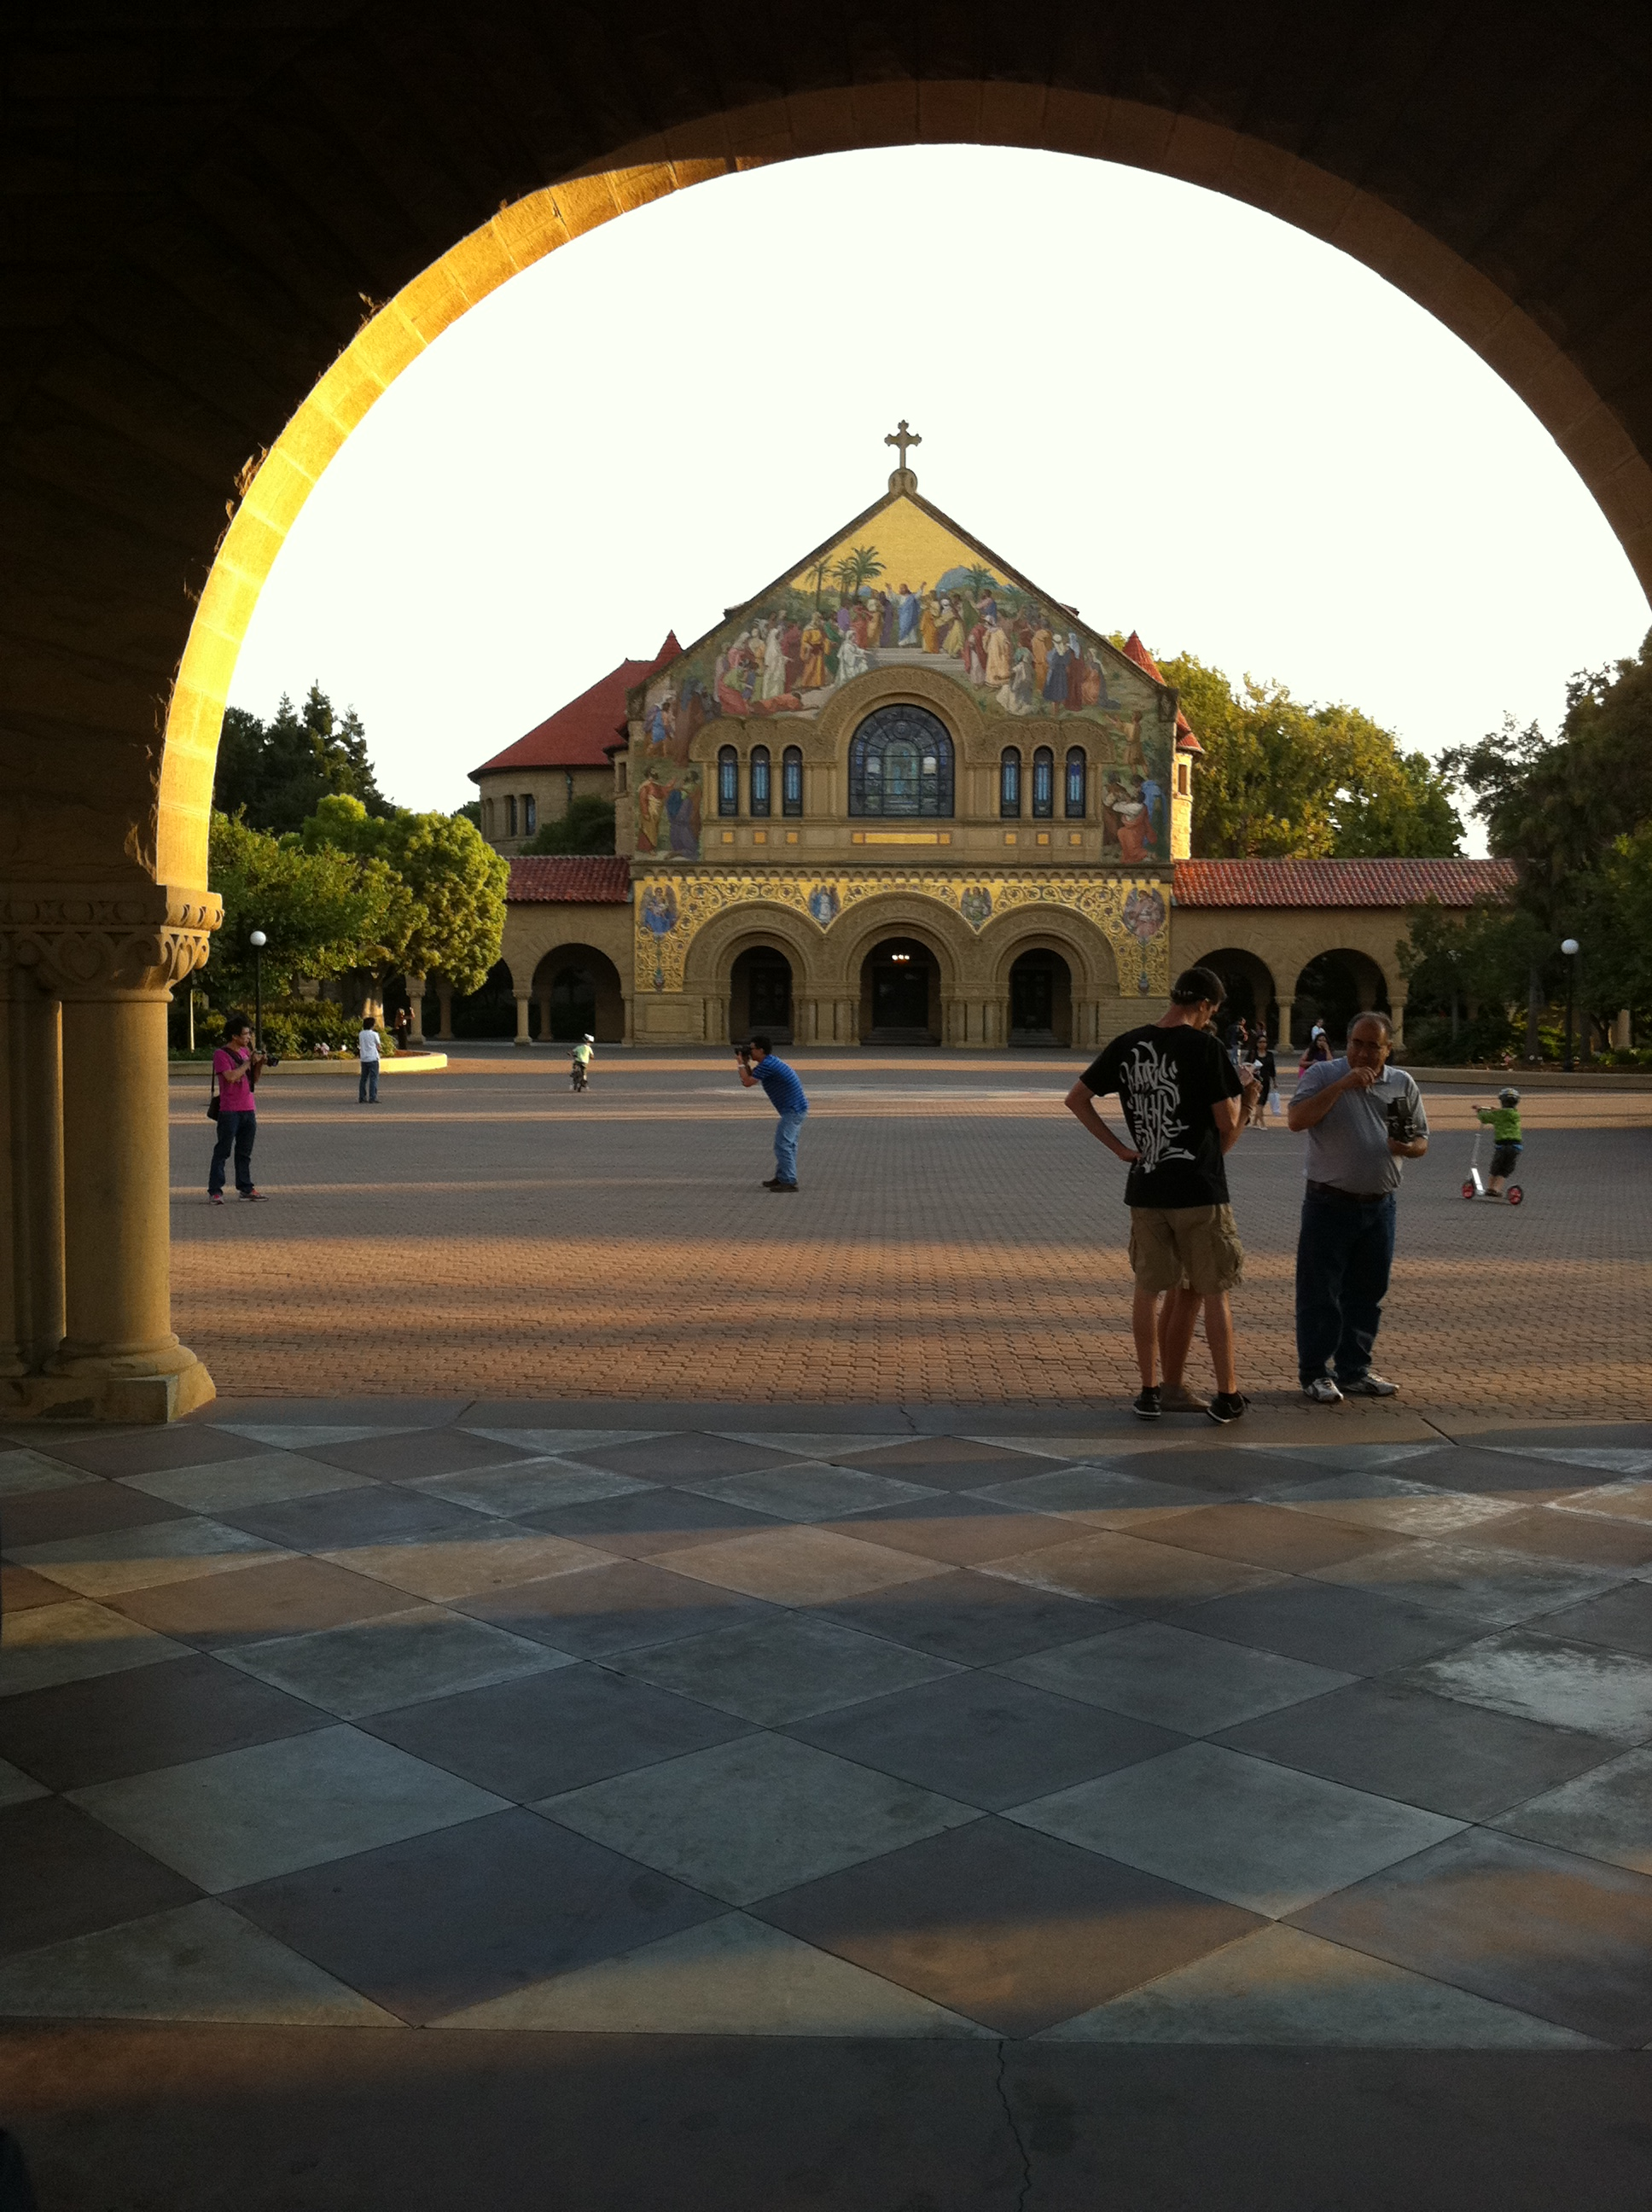
\includegraphics[width=\textwidth]{memchu.jpg}
                \caption{Taken clear image.}
        \end{subfigure}
        
        \vspace{1cm}
        \begin{subfigure}[b]{0.35\textwidth}
                 \centering
                 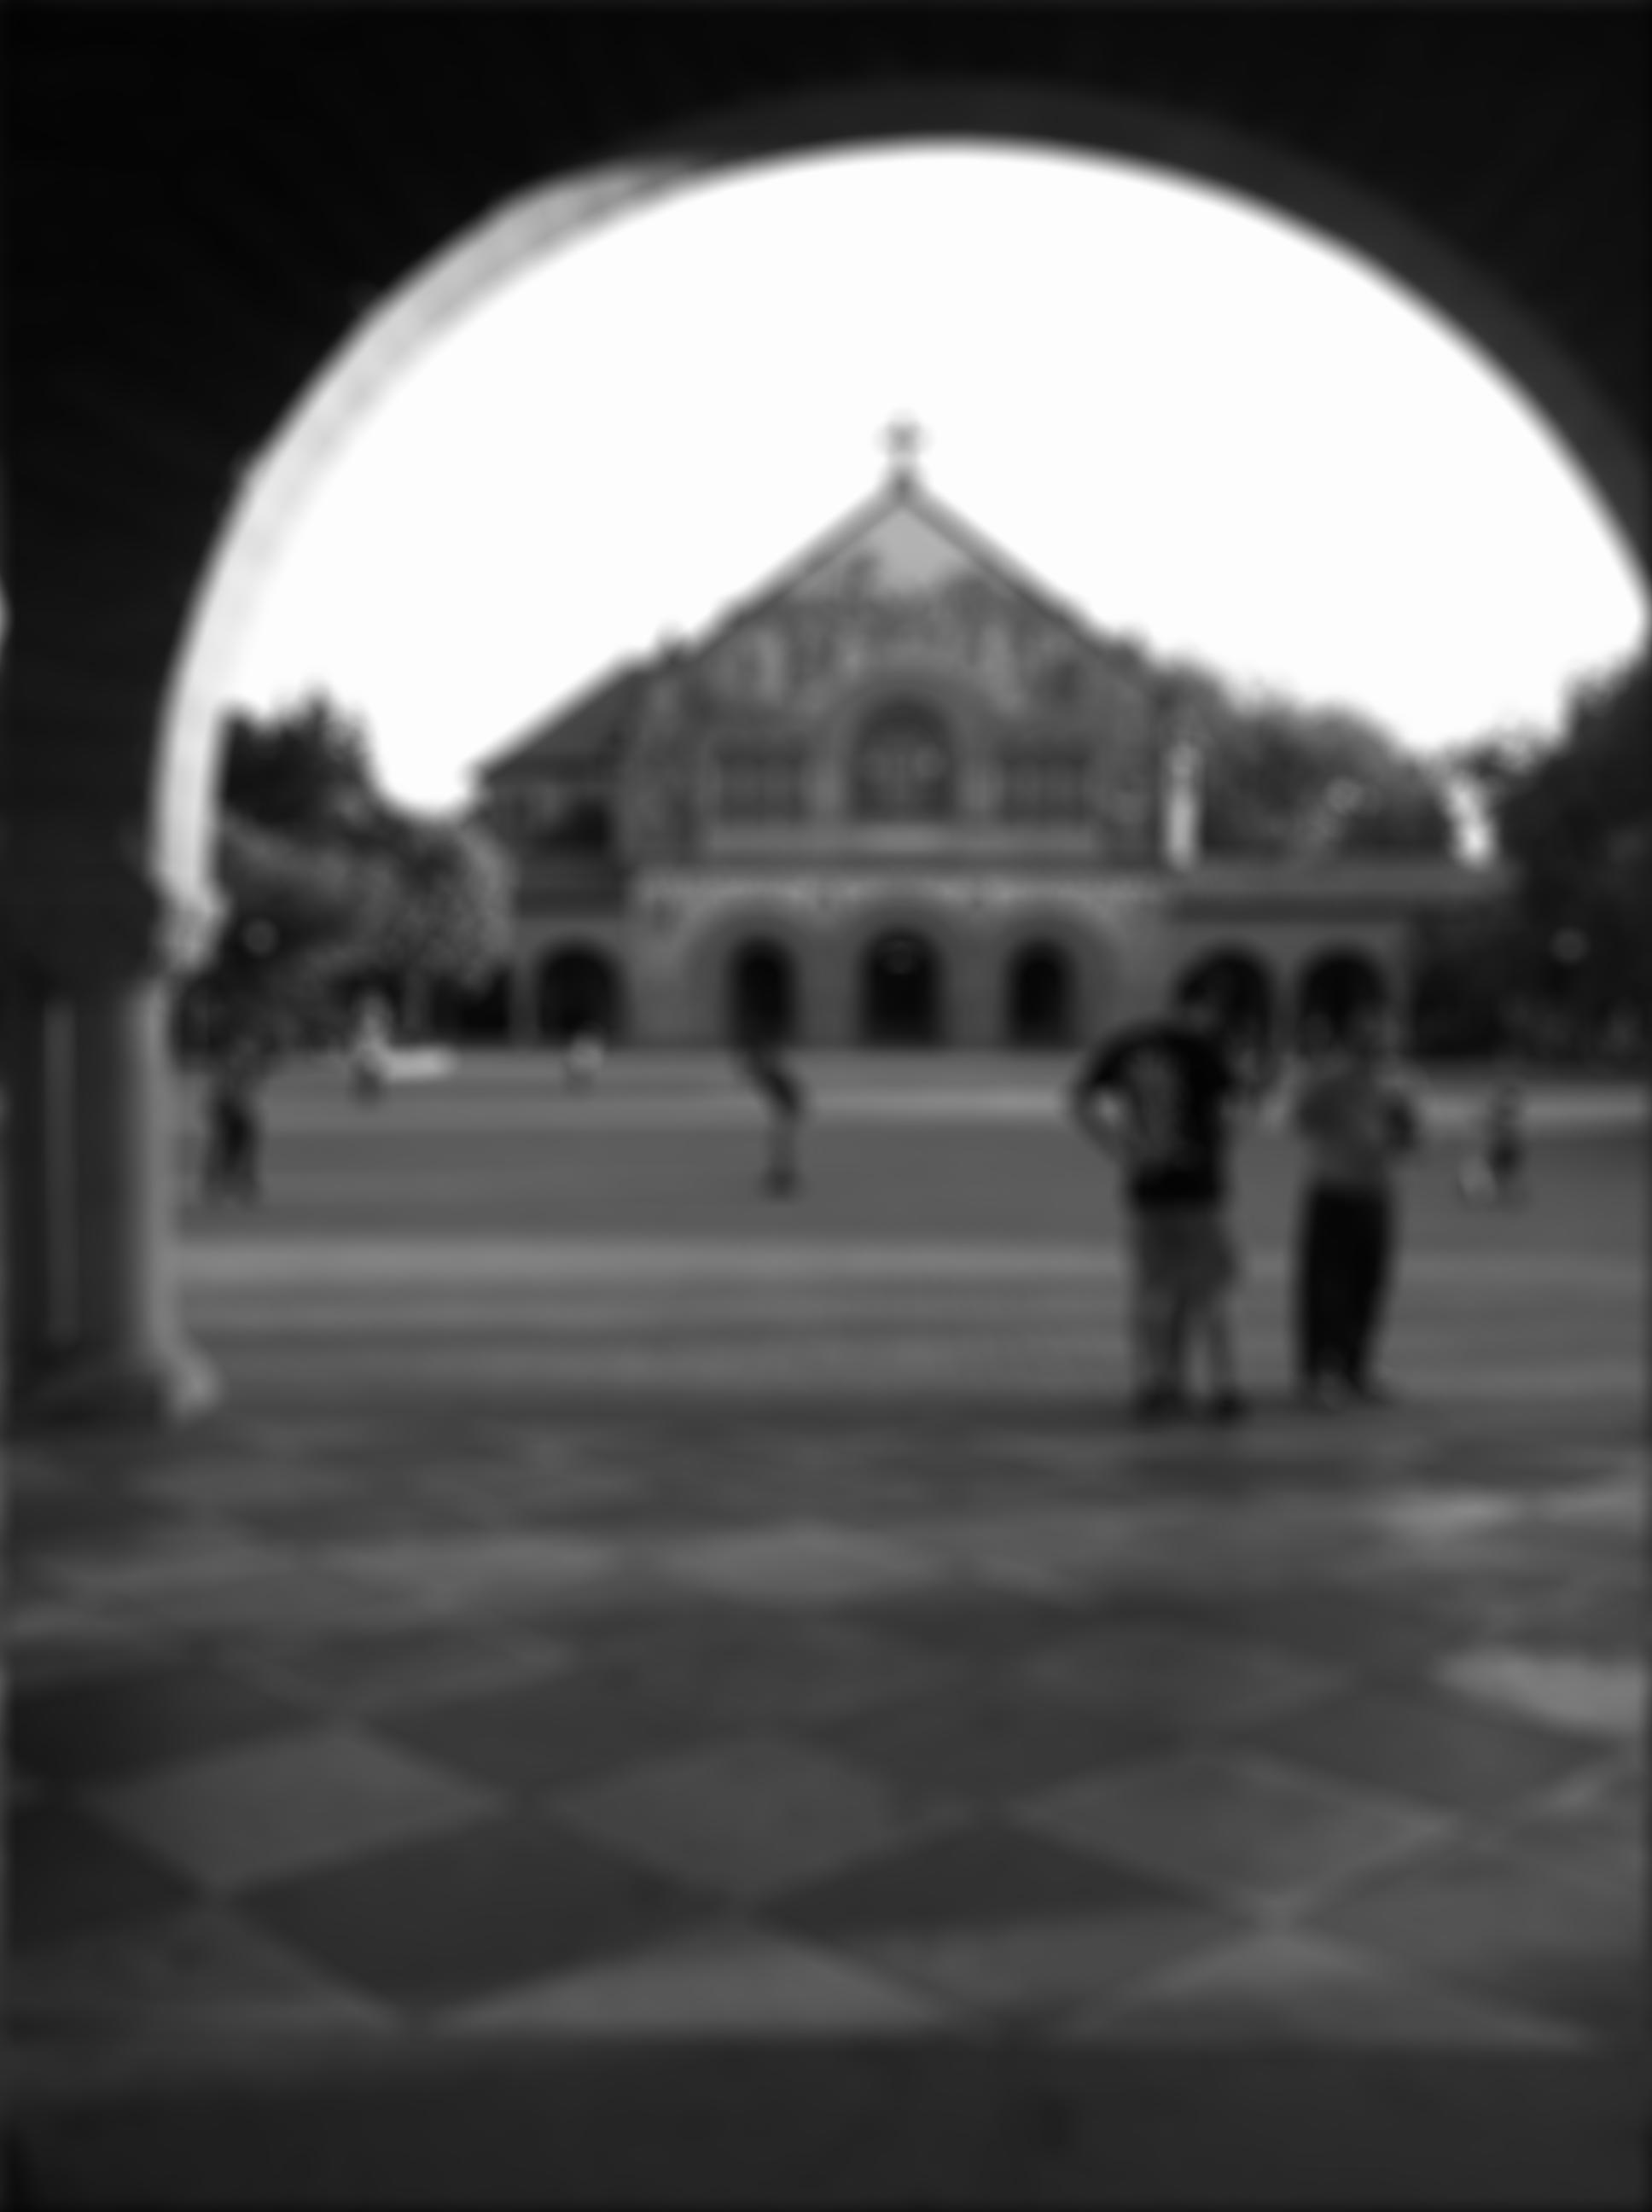
\includegraphics[width=\textwidth]{memchu_blur.jpg}
                 \caption{Image blurred using a disk kernel and without noise.}\label{fig:base_images_nonoise}
        \end{subfigure}  
        \hspace{1.5cm}
        \begin{subfigure}[b]{0.35\textwidth}
                         \centering
                         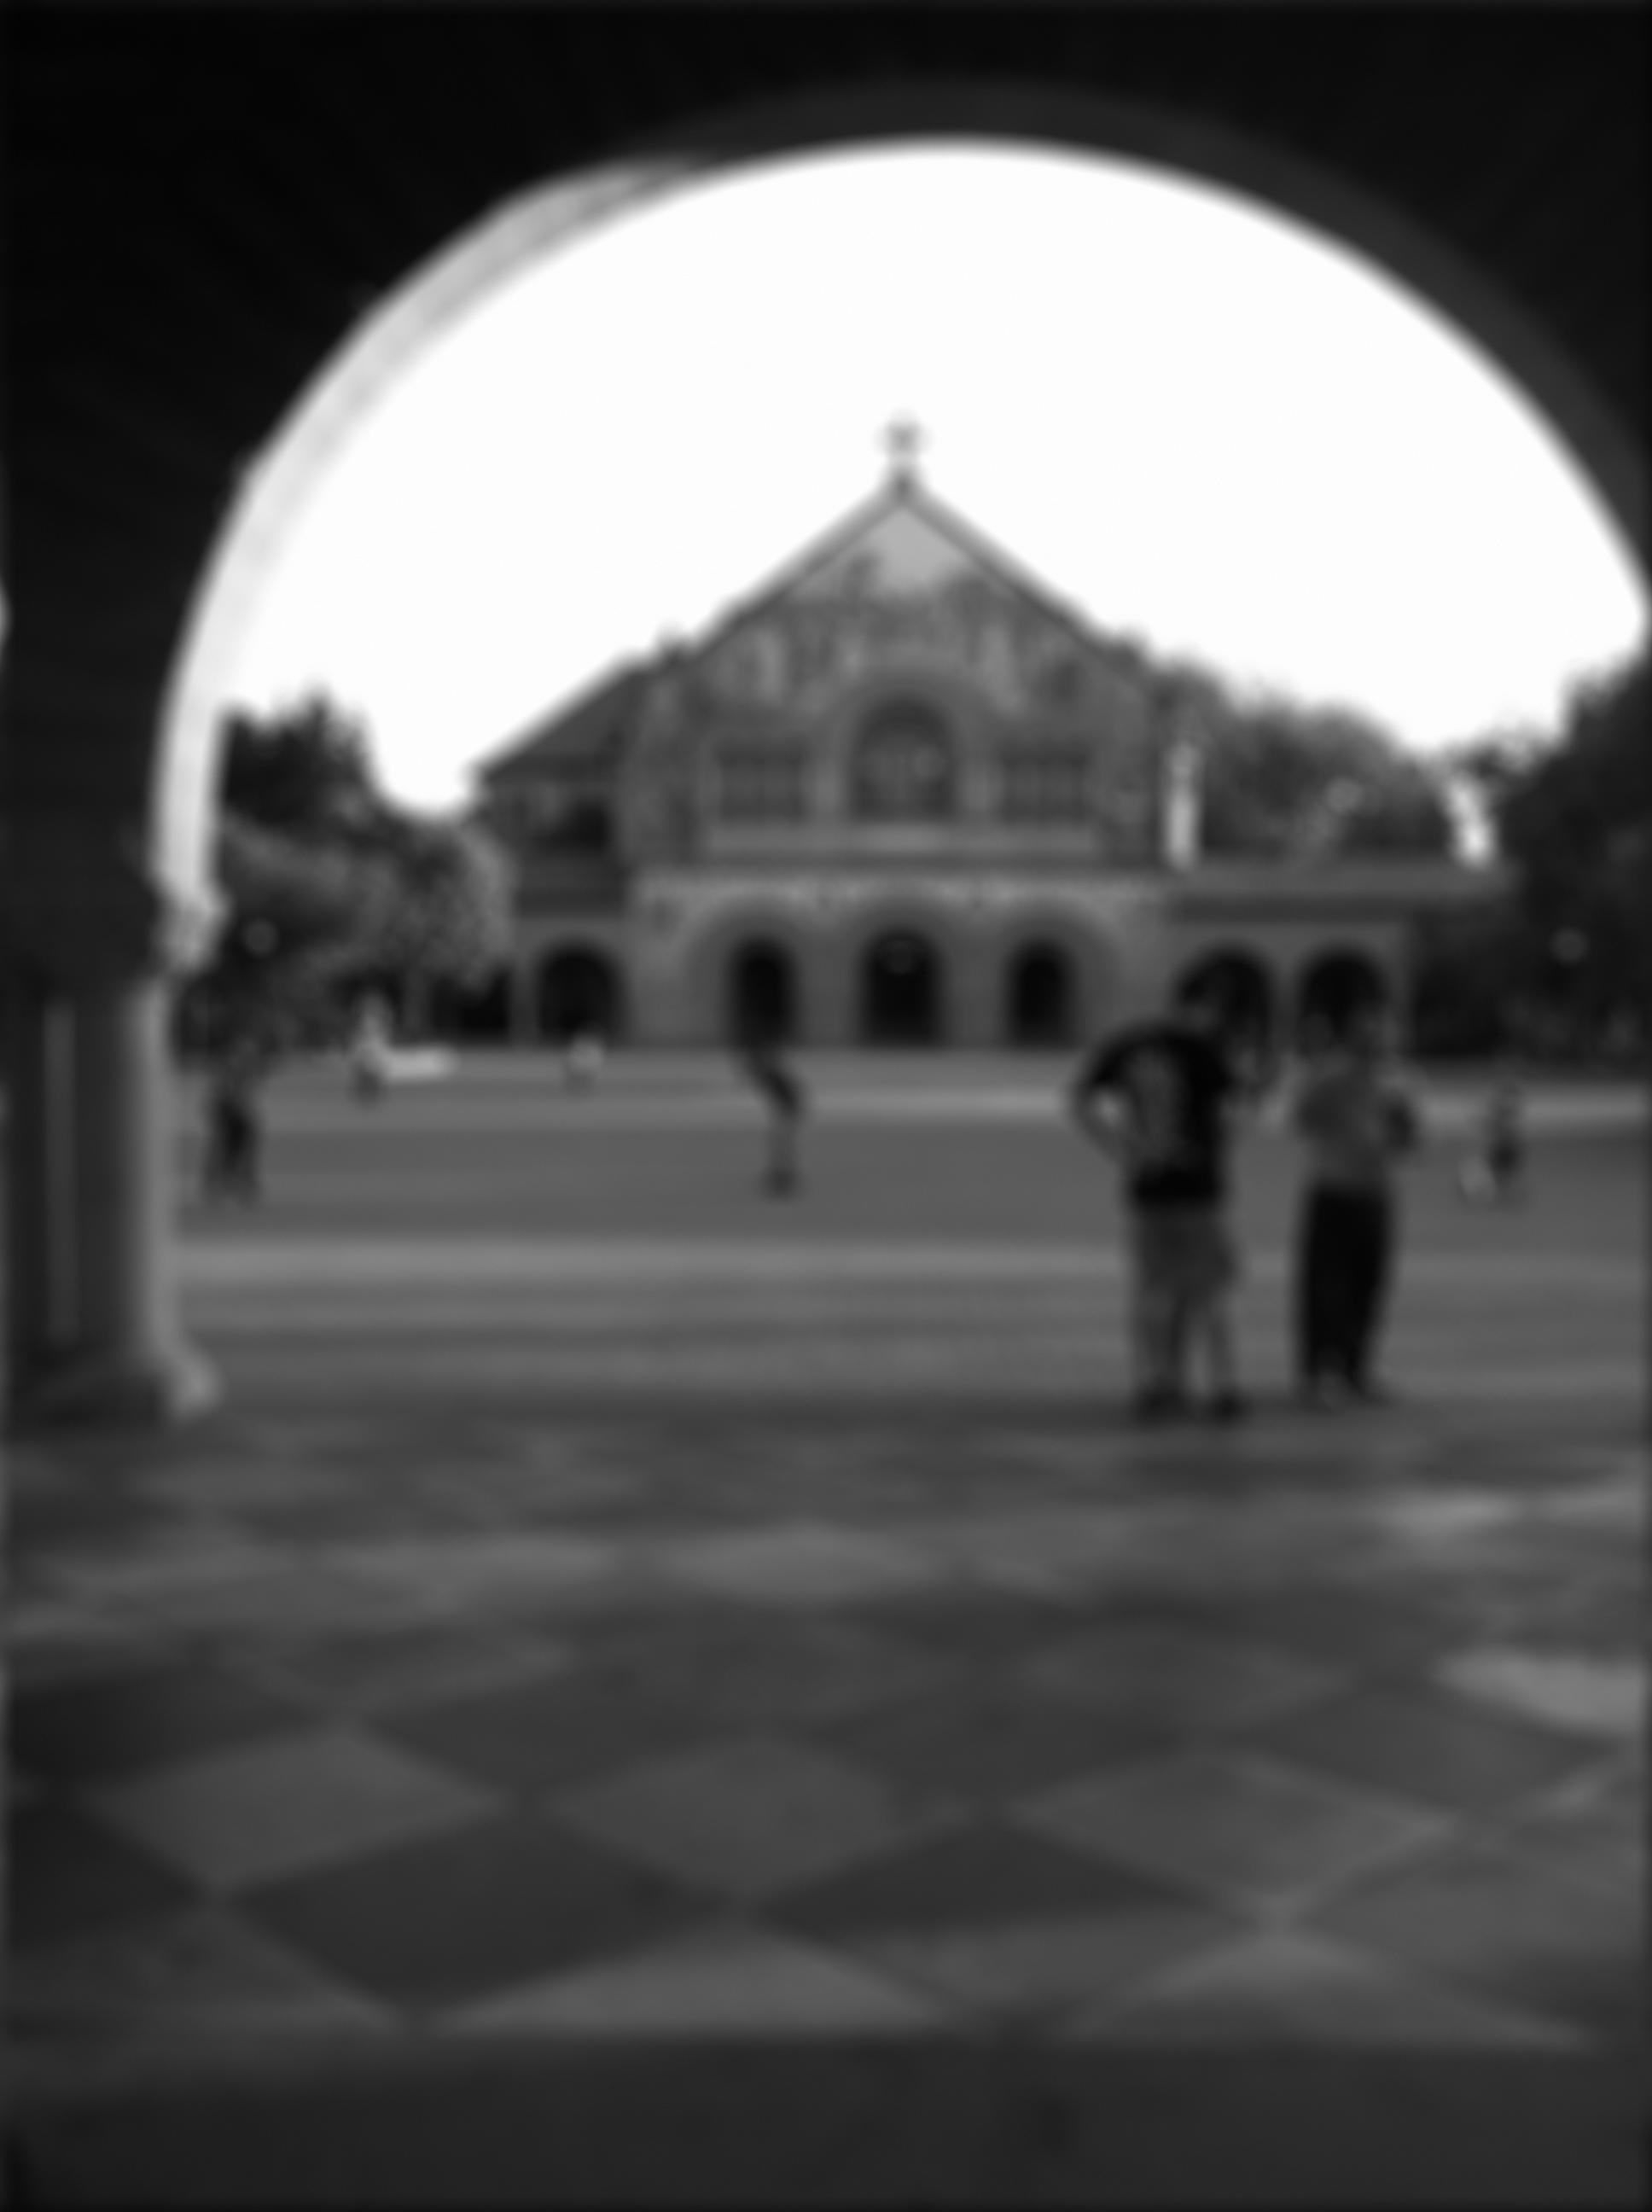
\includegraphics[width=\textwidth]{memchu_blur_noise.jpg}
                         \caption{Image blurred using a disk kernel and with noise variance set to $10^(-5)$  }\label{fig:base_images_noise}
        \end{subfigure}
        
        \caption{Images of the Memorial Church used to test the filters and the sharpness metrics.}
        \label{fig:base_images}
\end{figure}

\begin{figure}[H]
        \centering
        \begin{subfigure}[b]{0.35\textwidth}
                \centering
                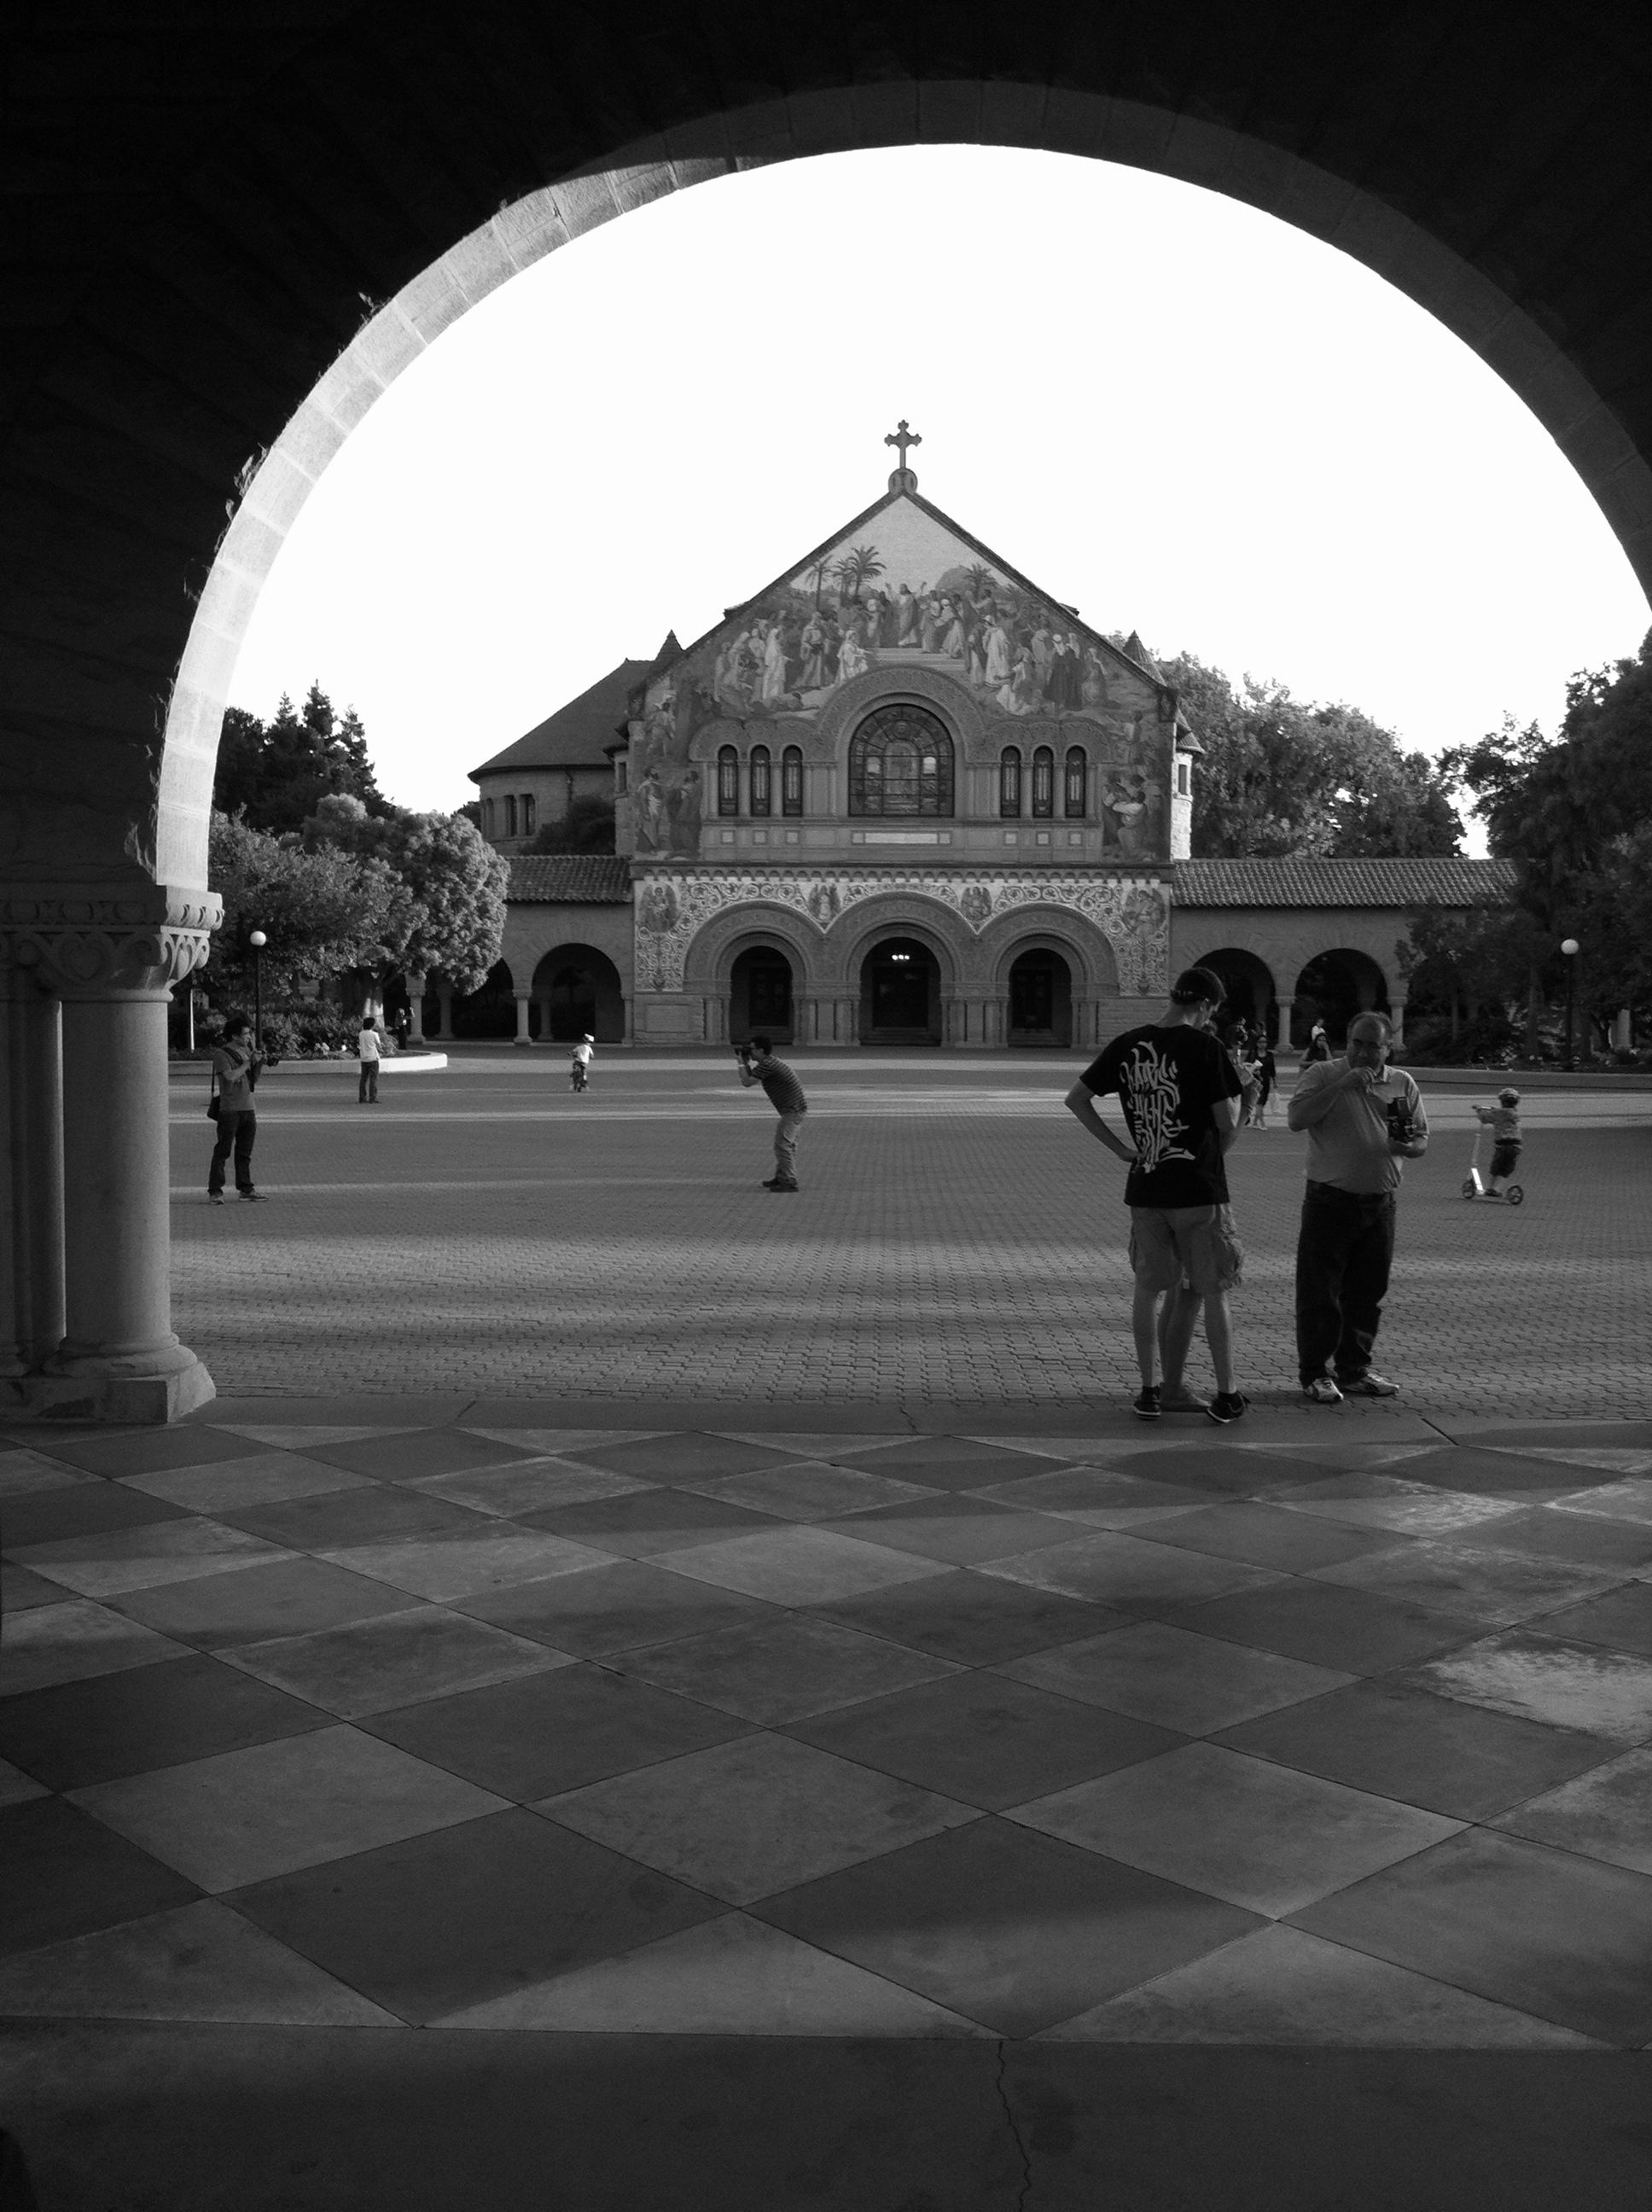
\includegraphics[width=\textwidth]{memchu_inv.jpg}
                \caption{Image obtained by using the Inverse filter.\newline $Grad=0.0170$ ; $SSI=1.000$ ; $JNB=68.849$}
        \end{subfigure}
        \hspace{1.5cm}
        \begin{subfigure}[b]{0.35\textwidth}
                 \centering
                 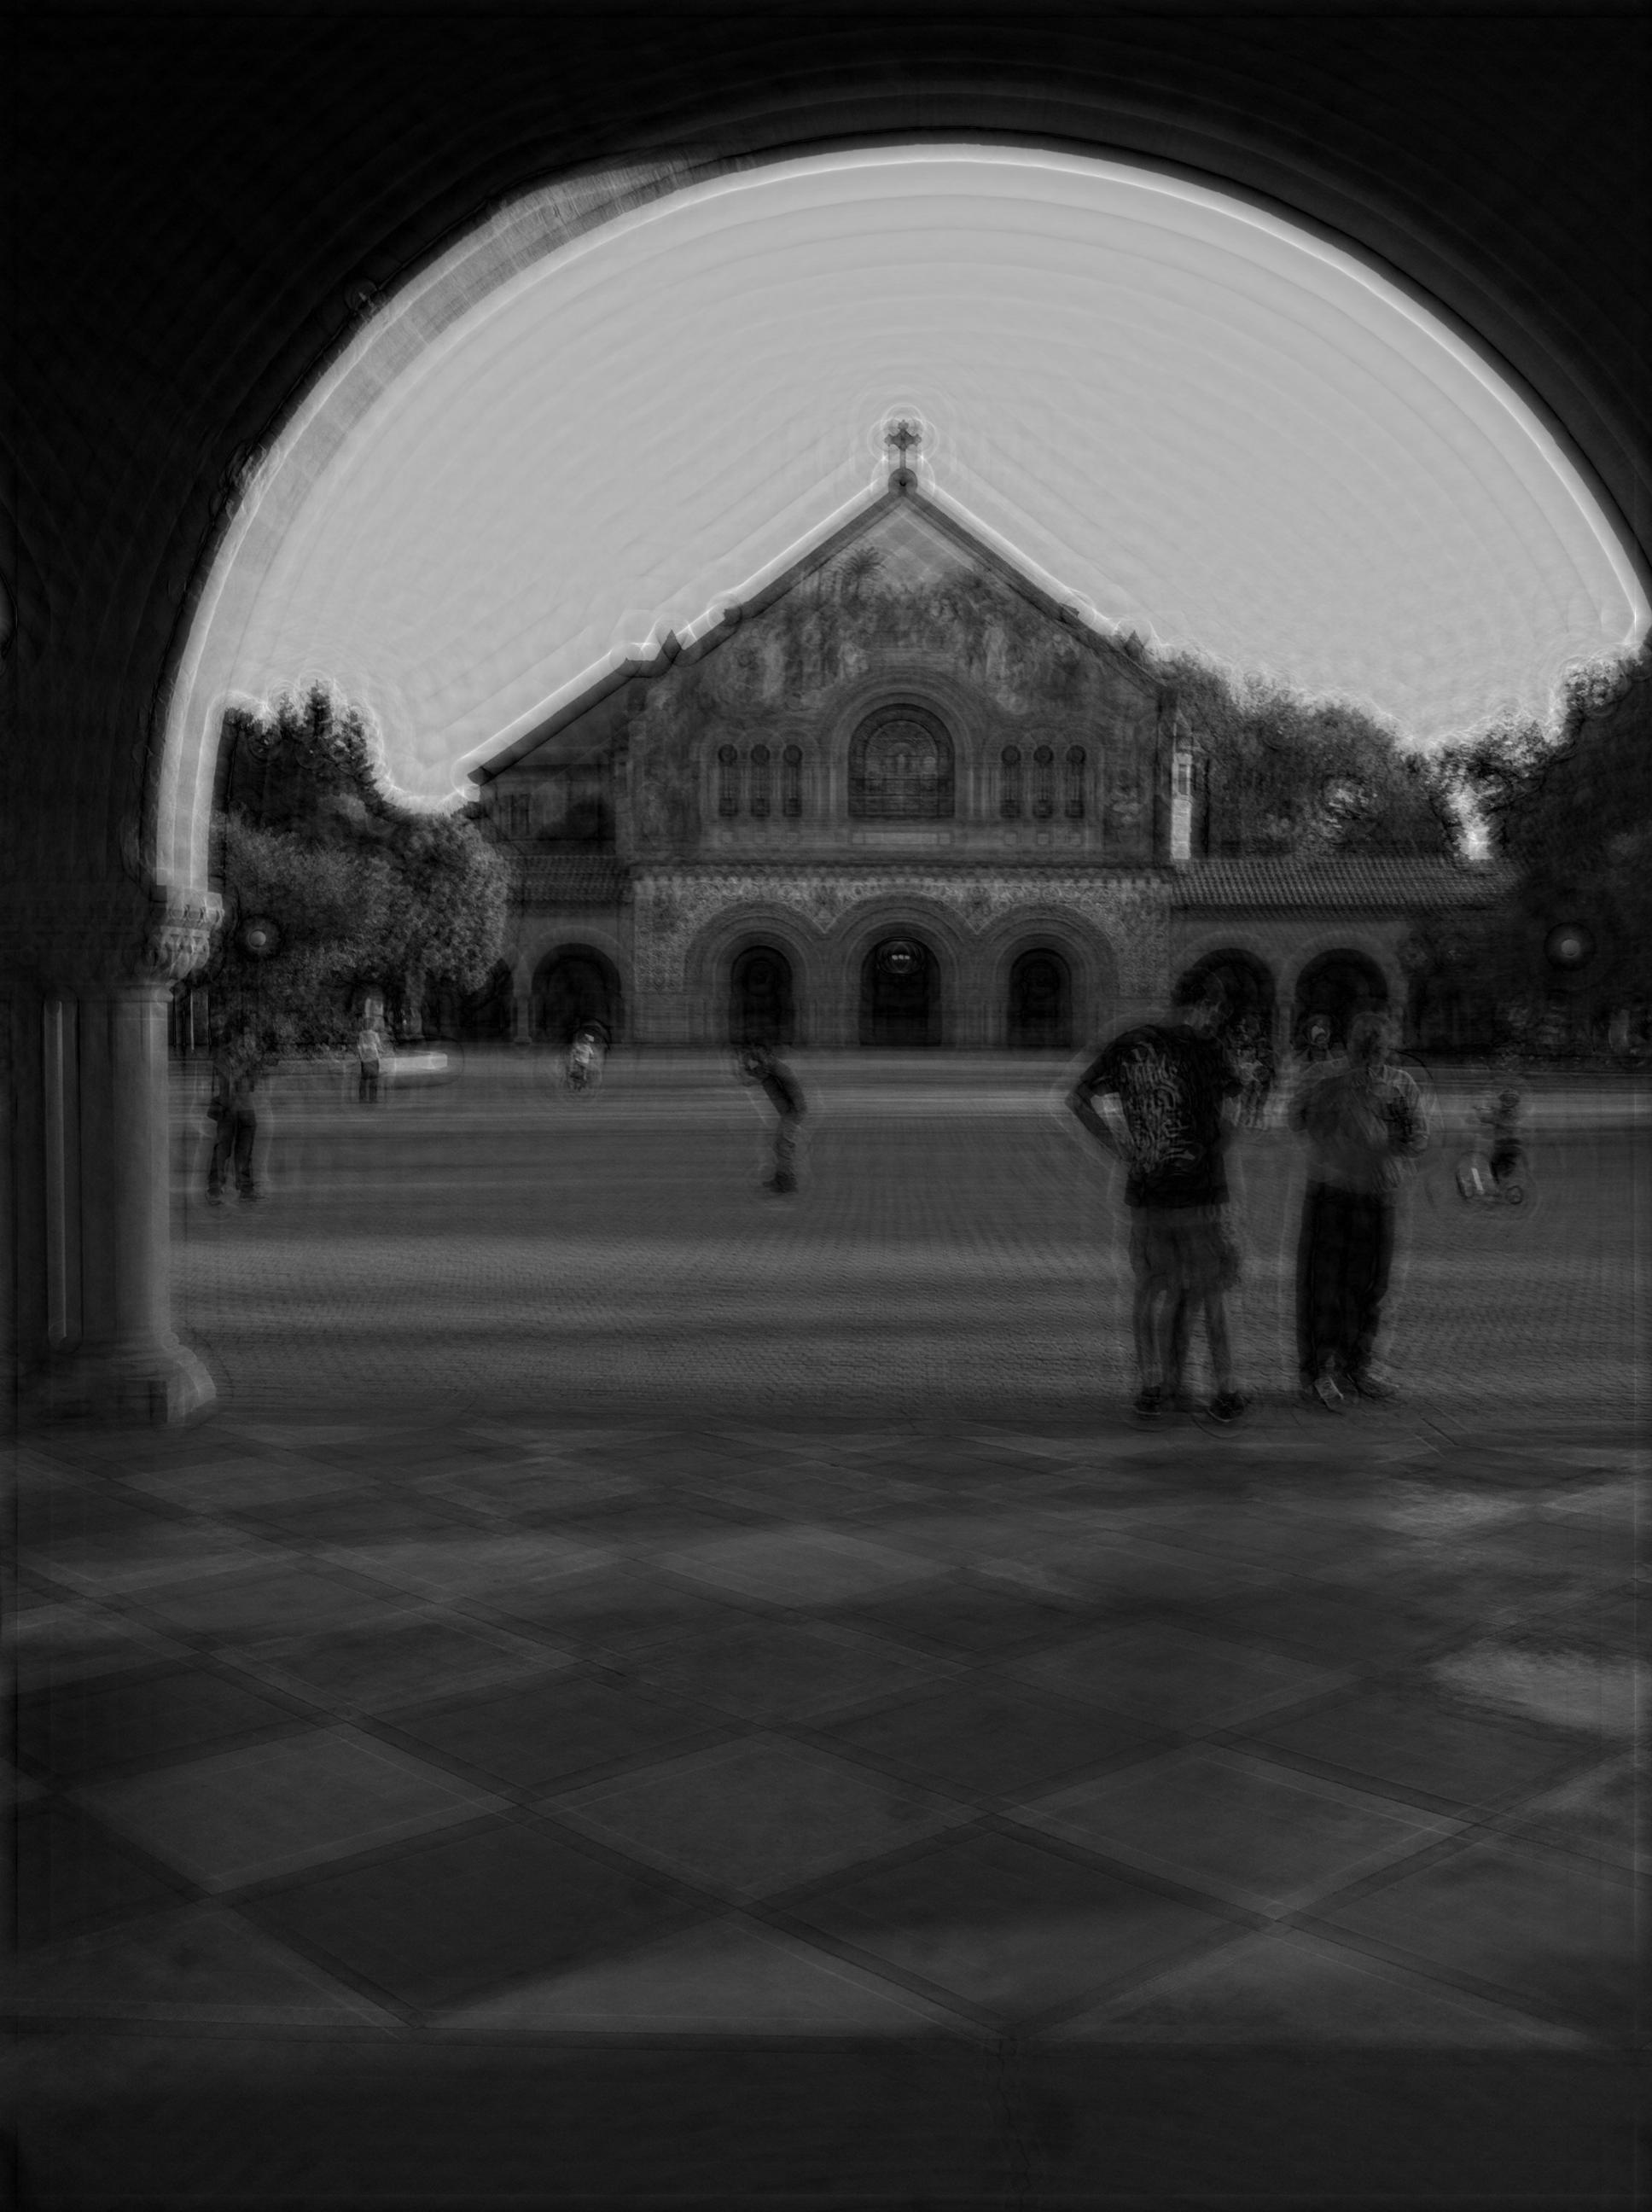
\includegraphics[width=\textwidth]{memchu_pinv.jpg}
                 \caption{Image obtained by using the Pseudo-Inverse filter.\newline $Grad=0.0102$ ; $SSI=0.9974$ ; $JNB=51.062$}
        \end{subfigure} 
        
         \vspace{1.5cm}
        \begin{subfigure}[b]{0.35\textwidth}
                        \centering
                        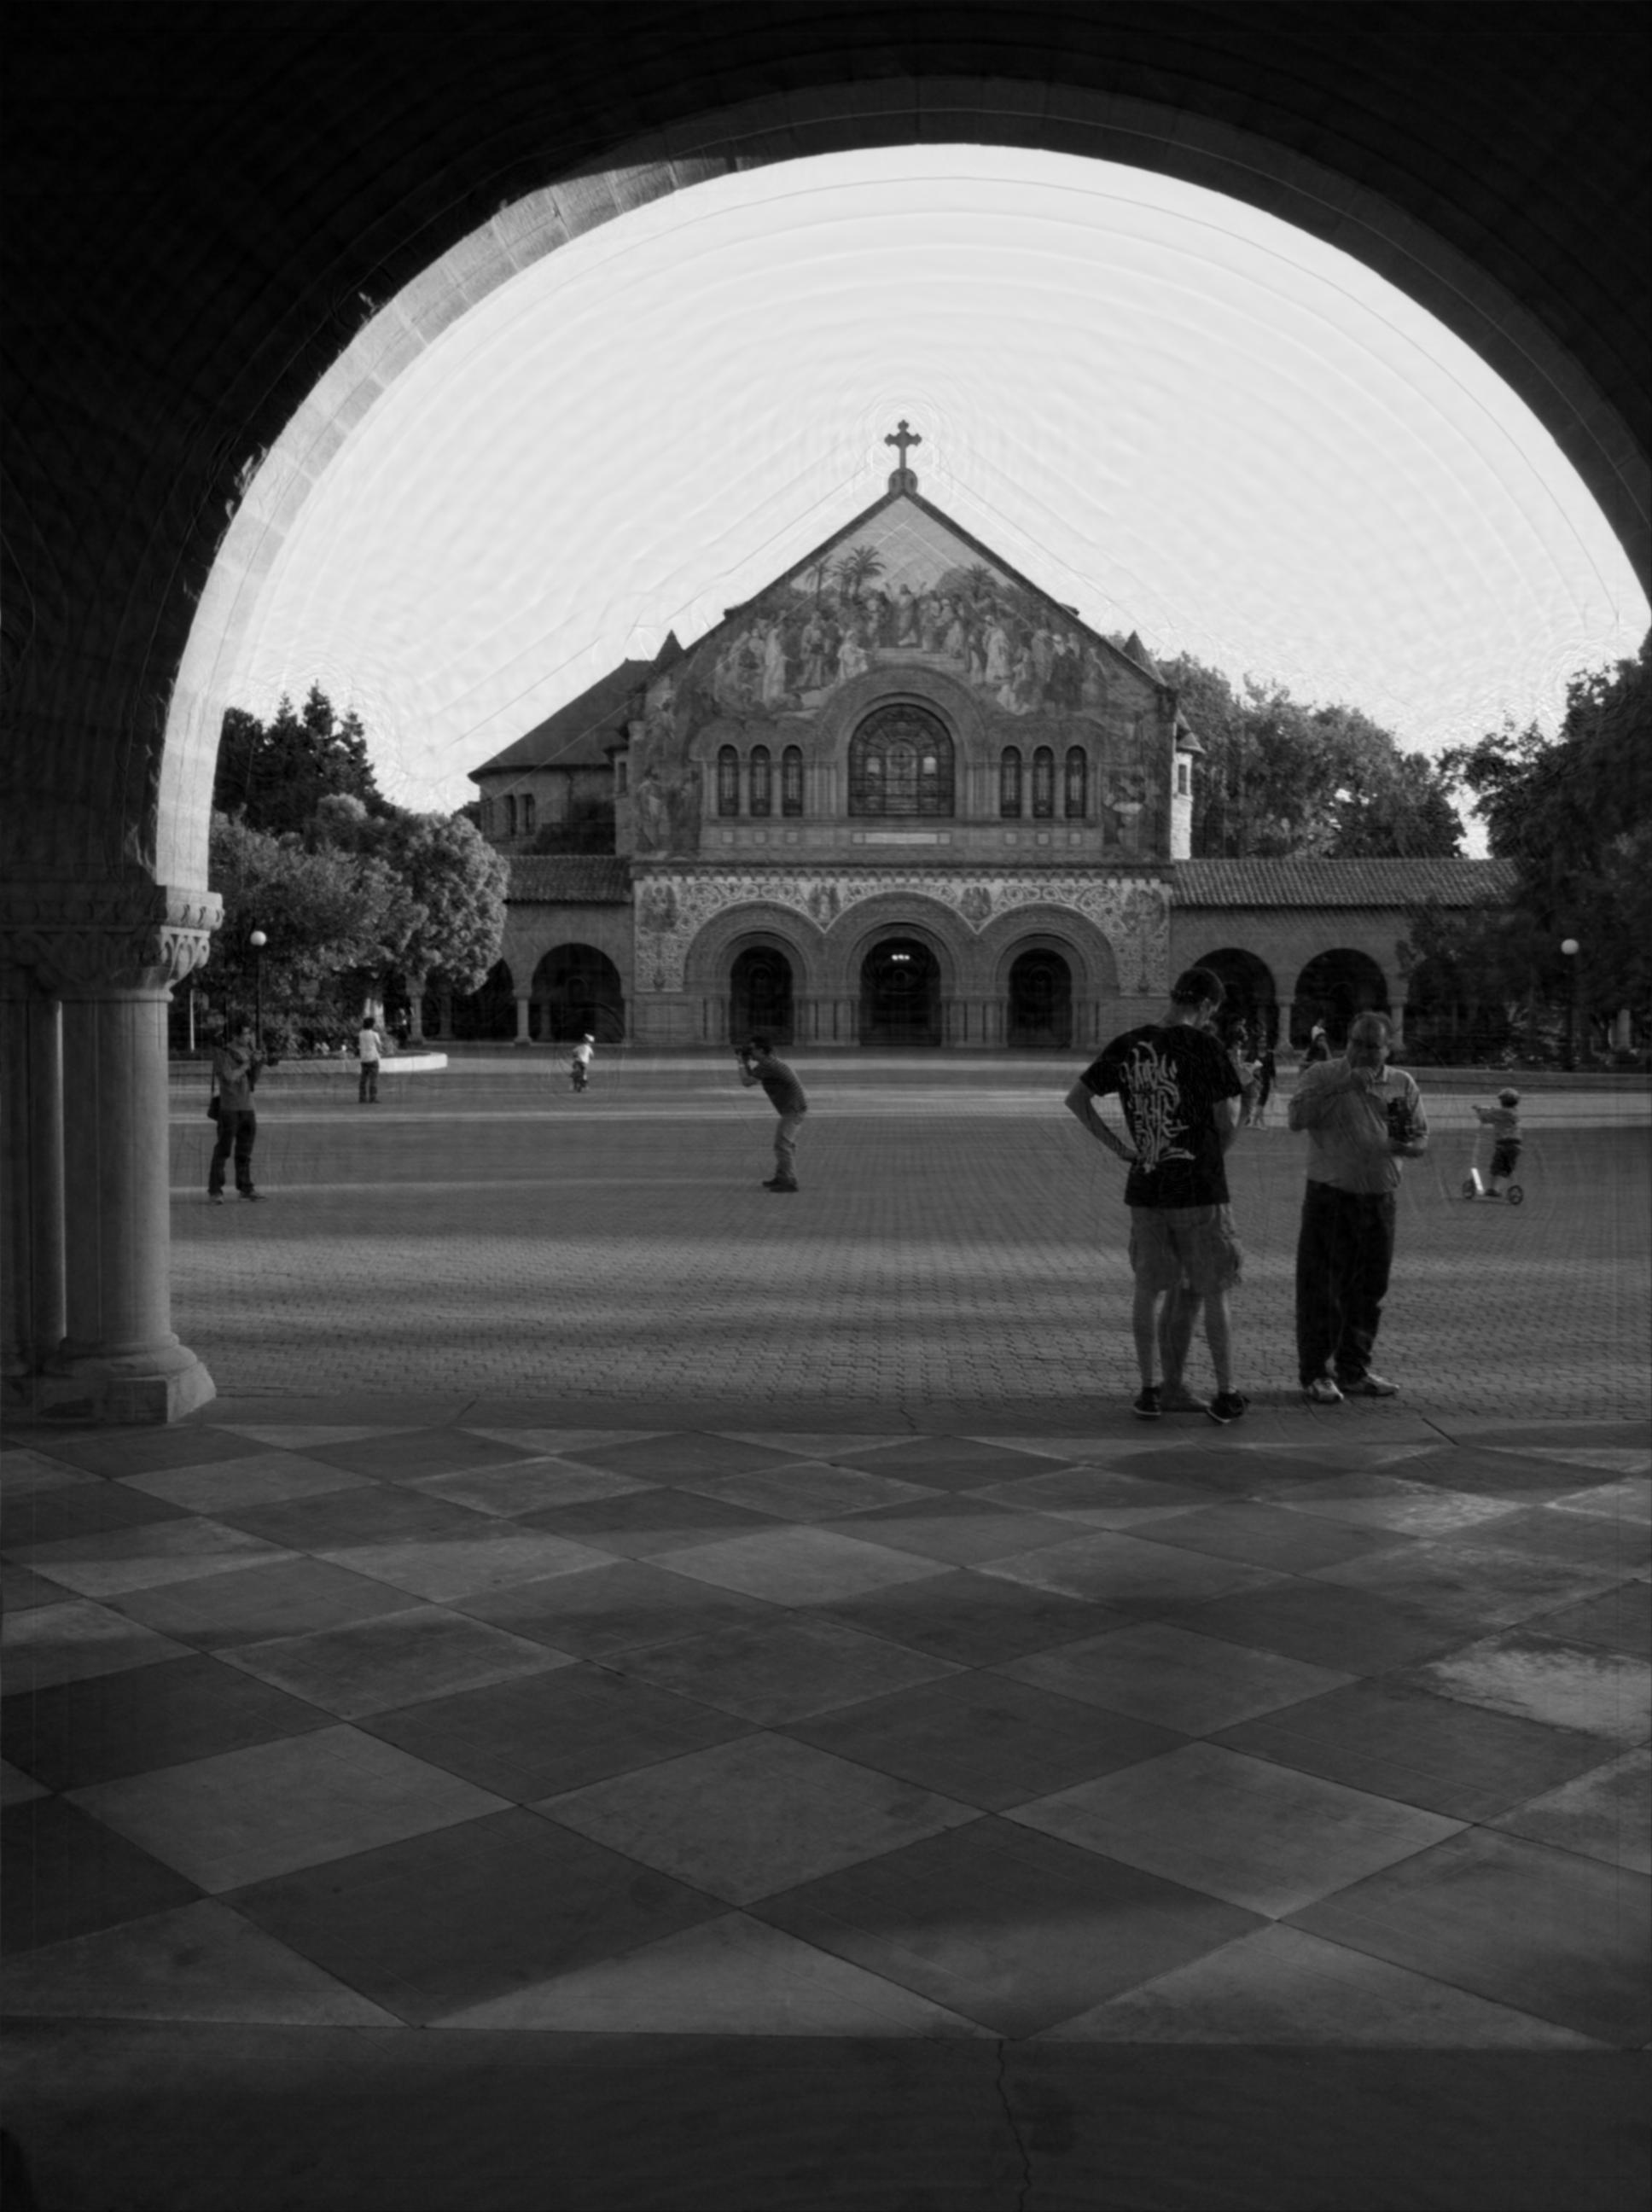
\includegraphics[width=\textwidth]{memchu_wiener.jpg}
                        \caption{Image obtained by using the Wiener filter.\newline $Grad=0.0085$ ; $SSI=0.9996$ ; $JNB=31.817$}
        \end{subfigure}
        \hspace{1cm}
        \begin{subfigure}[b]{0.35\textwidth}
                        \centering
                         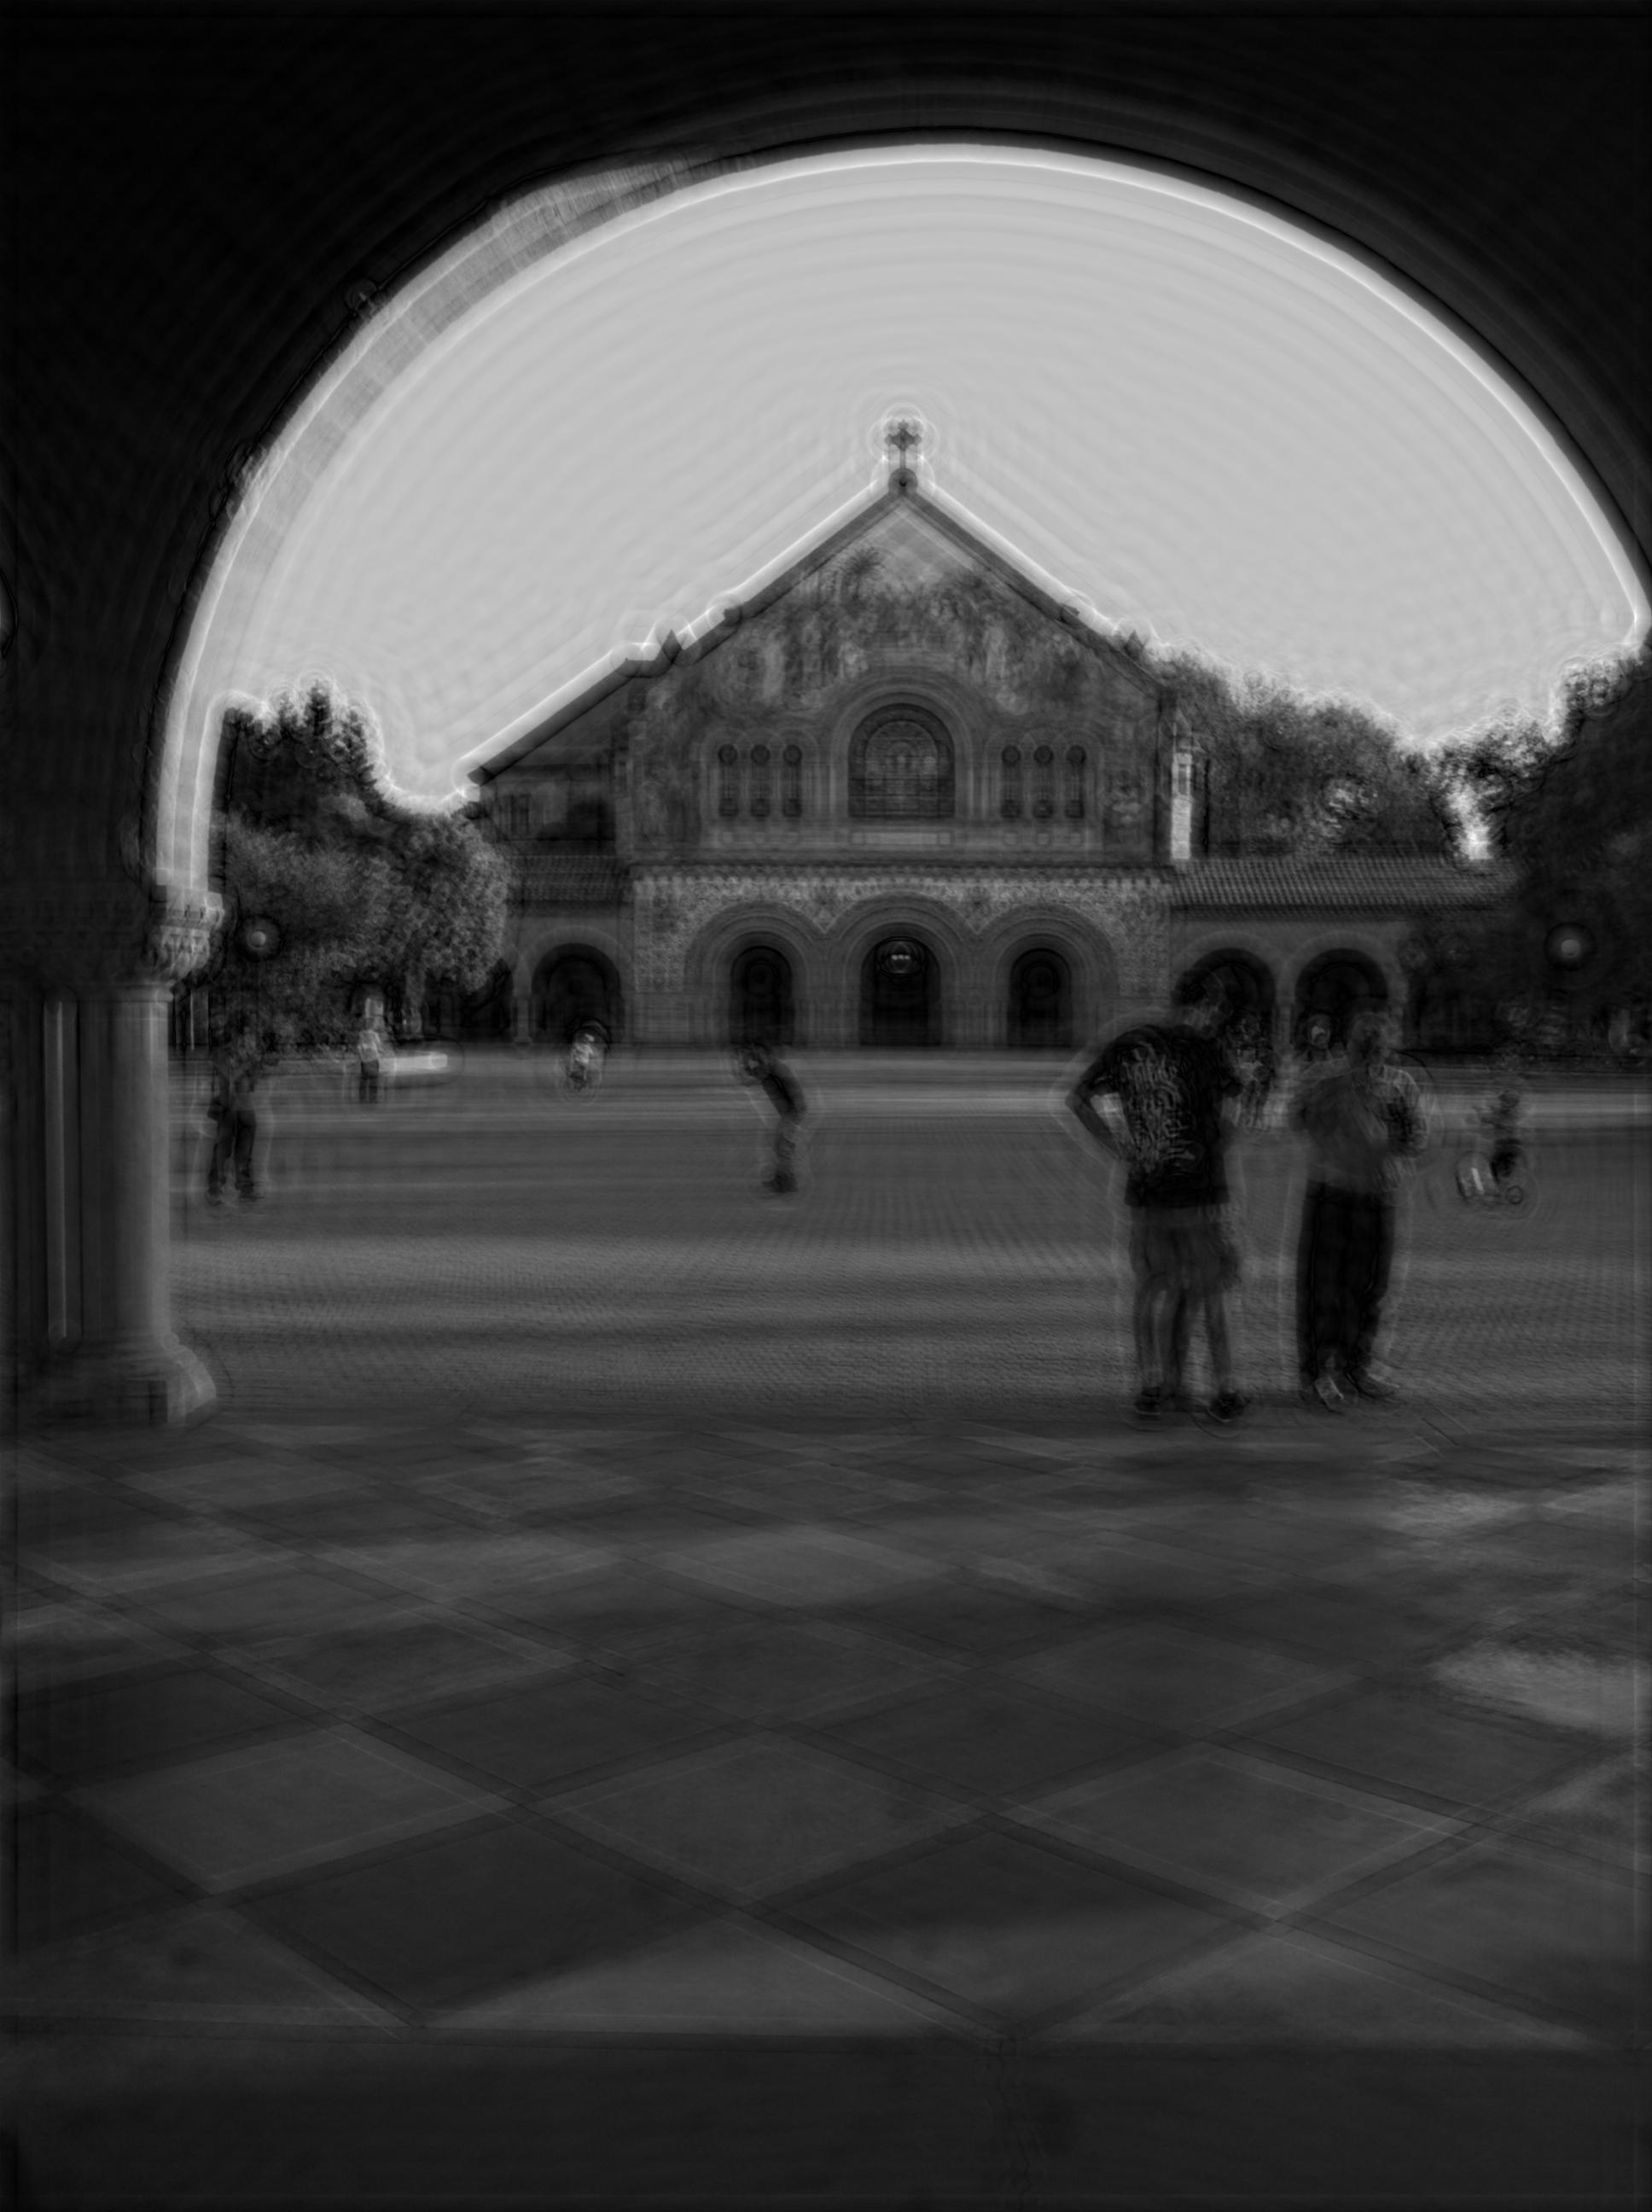
\includegraphics[width=\textwidth]{memchu_geo.jpg}
                         \caption{Image obtained by using the geometric mean filter.\newline $Grad=0.0072$ ; $SSI=0.9981$ ; $JNB=28.798$}
        \end{subfigure} 
        
        \caption{Recovered images using various filters starting with a blurry image without noise (Figure~\ref{fig:base_images_nonoise}).}
        \label{filtered_images_nonoise}
\end{figure}

\begin{figure}[H]
        \centering
        \begin{subfigure}[b]{0.35\textwidth}
                \centering
                
\includegraphics[width=\textwidth]{memchu_inv_noise.jpg}
                \caption{Image obtained by using the Inverse filter.\newline $Grad=0.1614$ ; $SSI=0.9866$ ; $JNB=121.289$}
        \end{subfigure}
        \hspace{1.5cm}
        \begin{subfigure}[b]{0.35\textwidth}
                 \centering
                 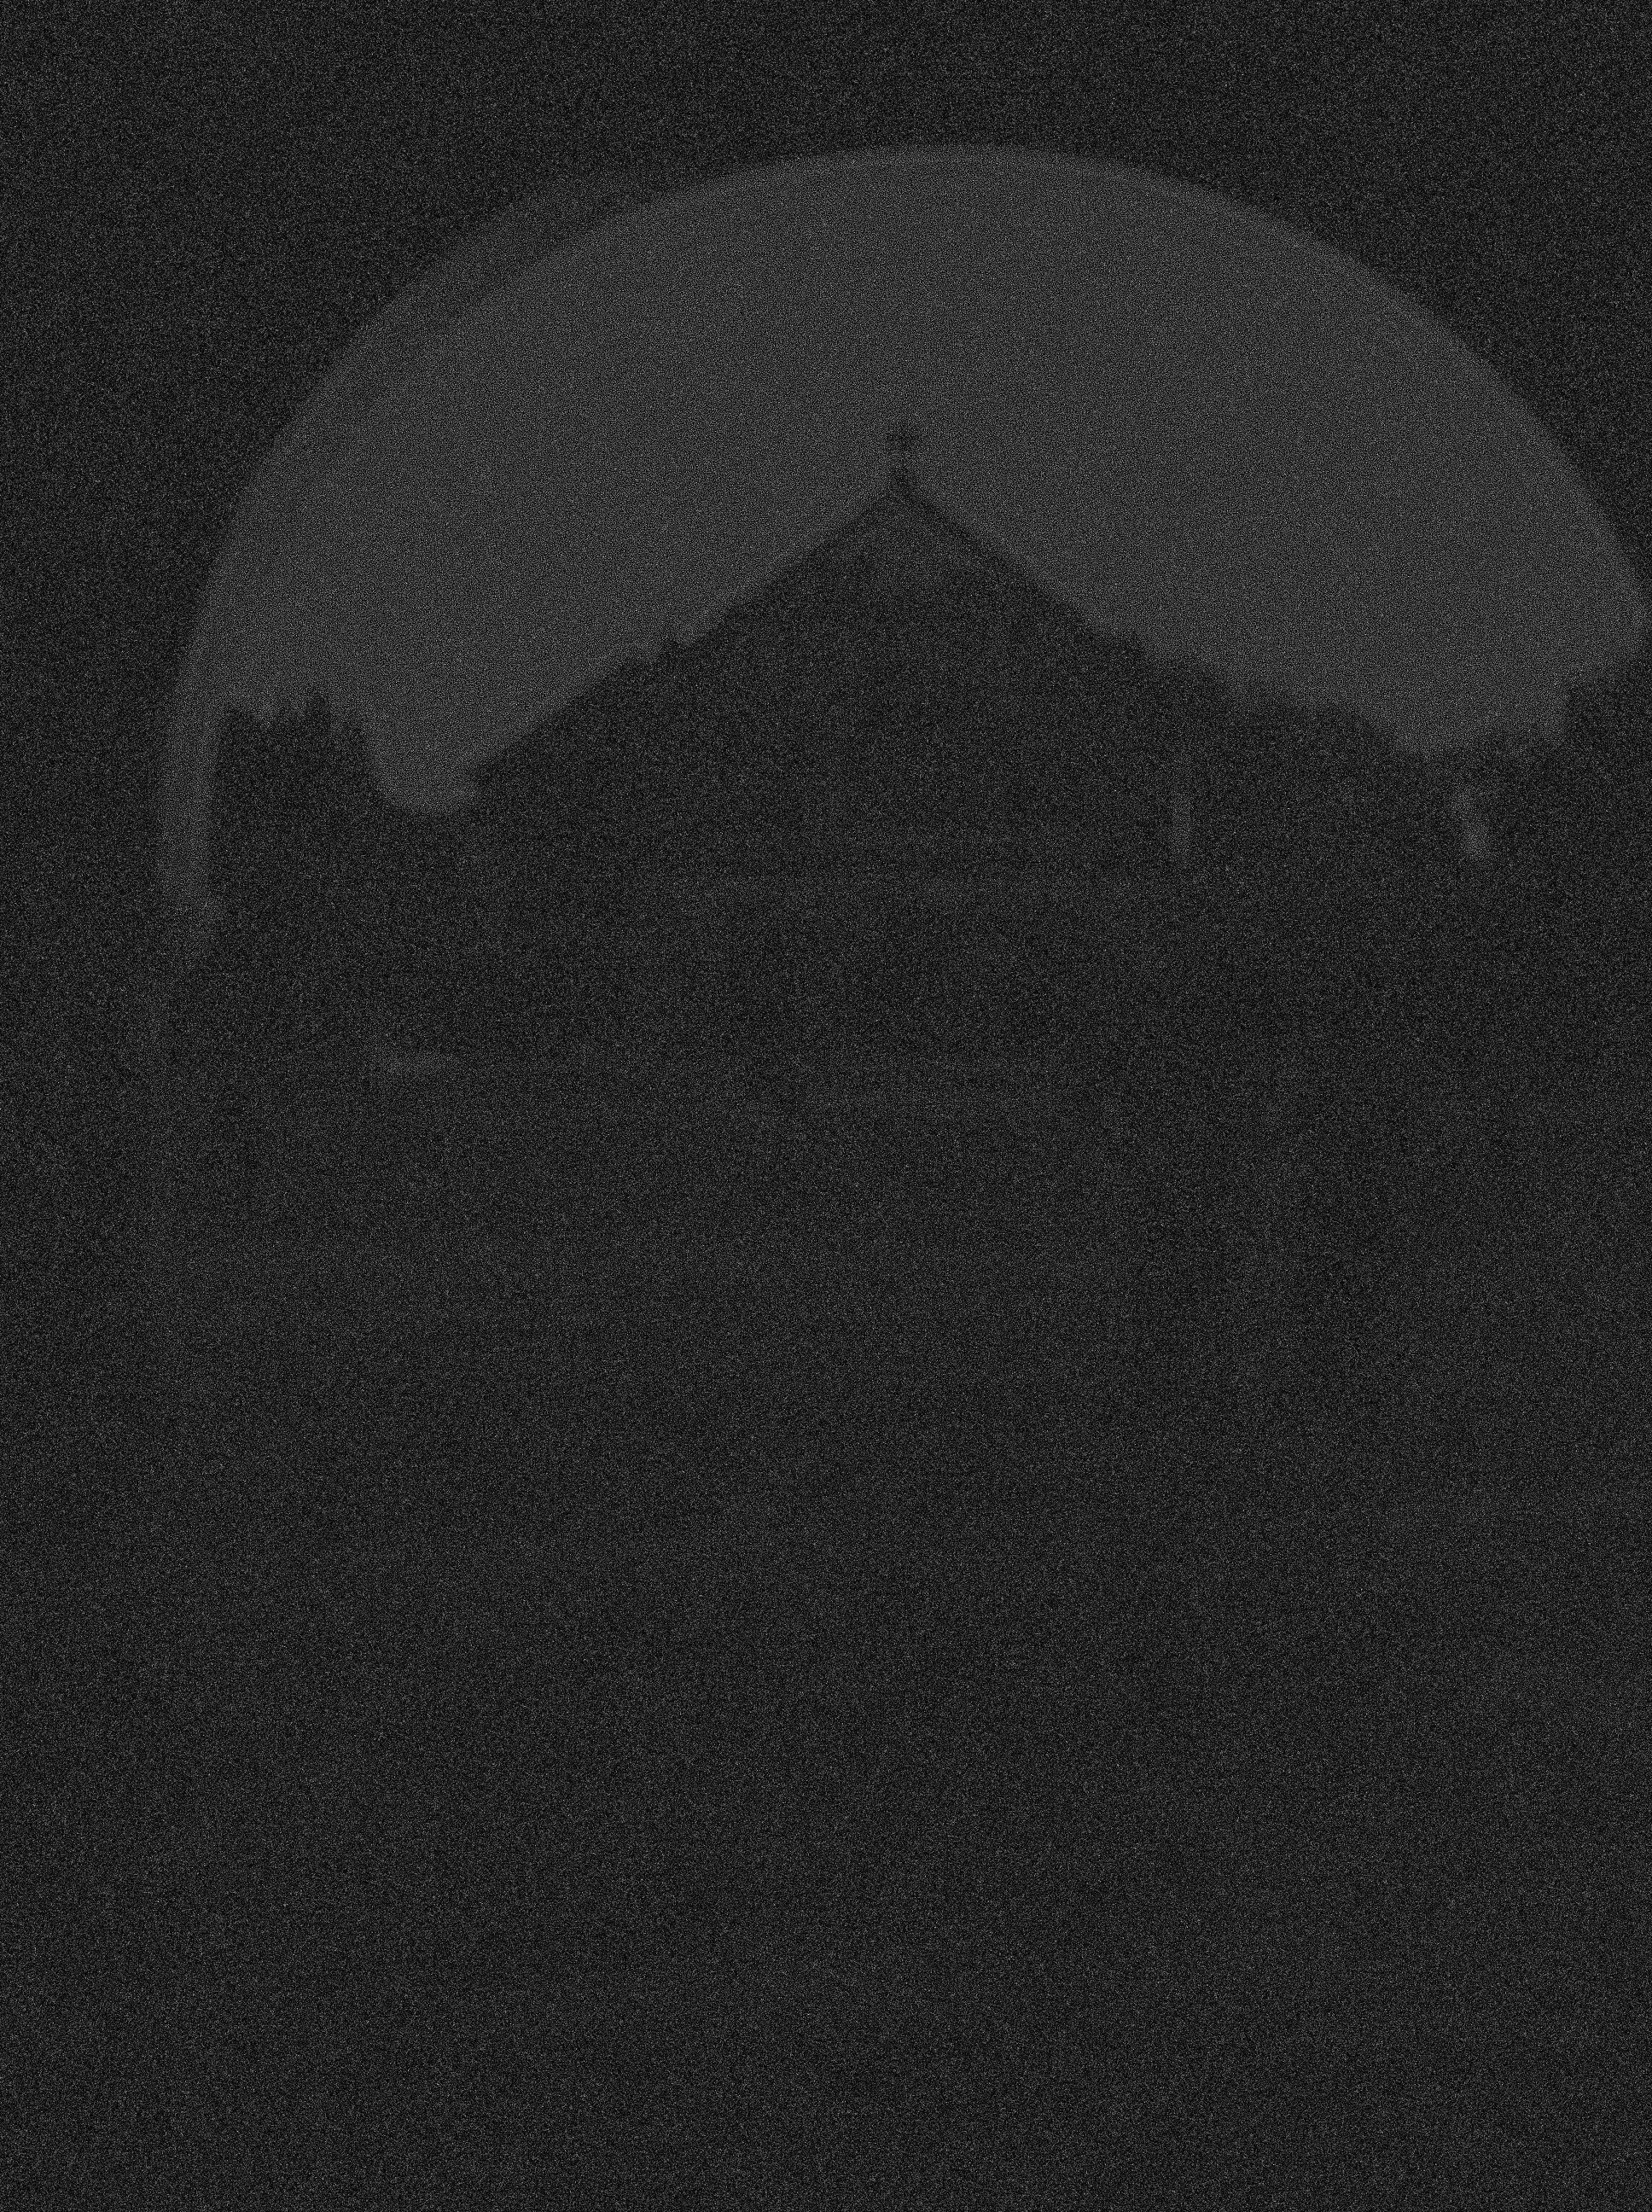
\includegraphics[width=\textwidth]{memchu_pinv_noise.jpg}
                 \caption{Image obtained by using the Pseudo-Inverse filter.\newline $Grad=0.0933$ ; $SSI=0.9831$ ; $JNB=97.711$}
        \end{subfigure} 
        
         \vspace{1.5cm}
        \begin{subfigure}[b]{0.35\textwidth}
                        \centering
                        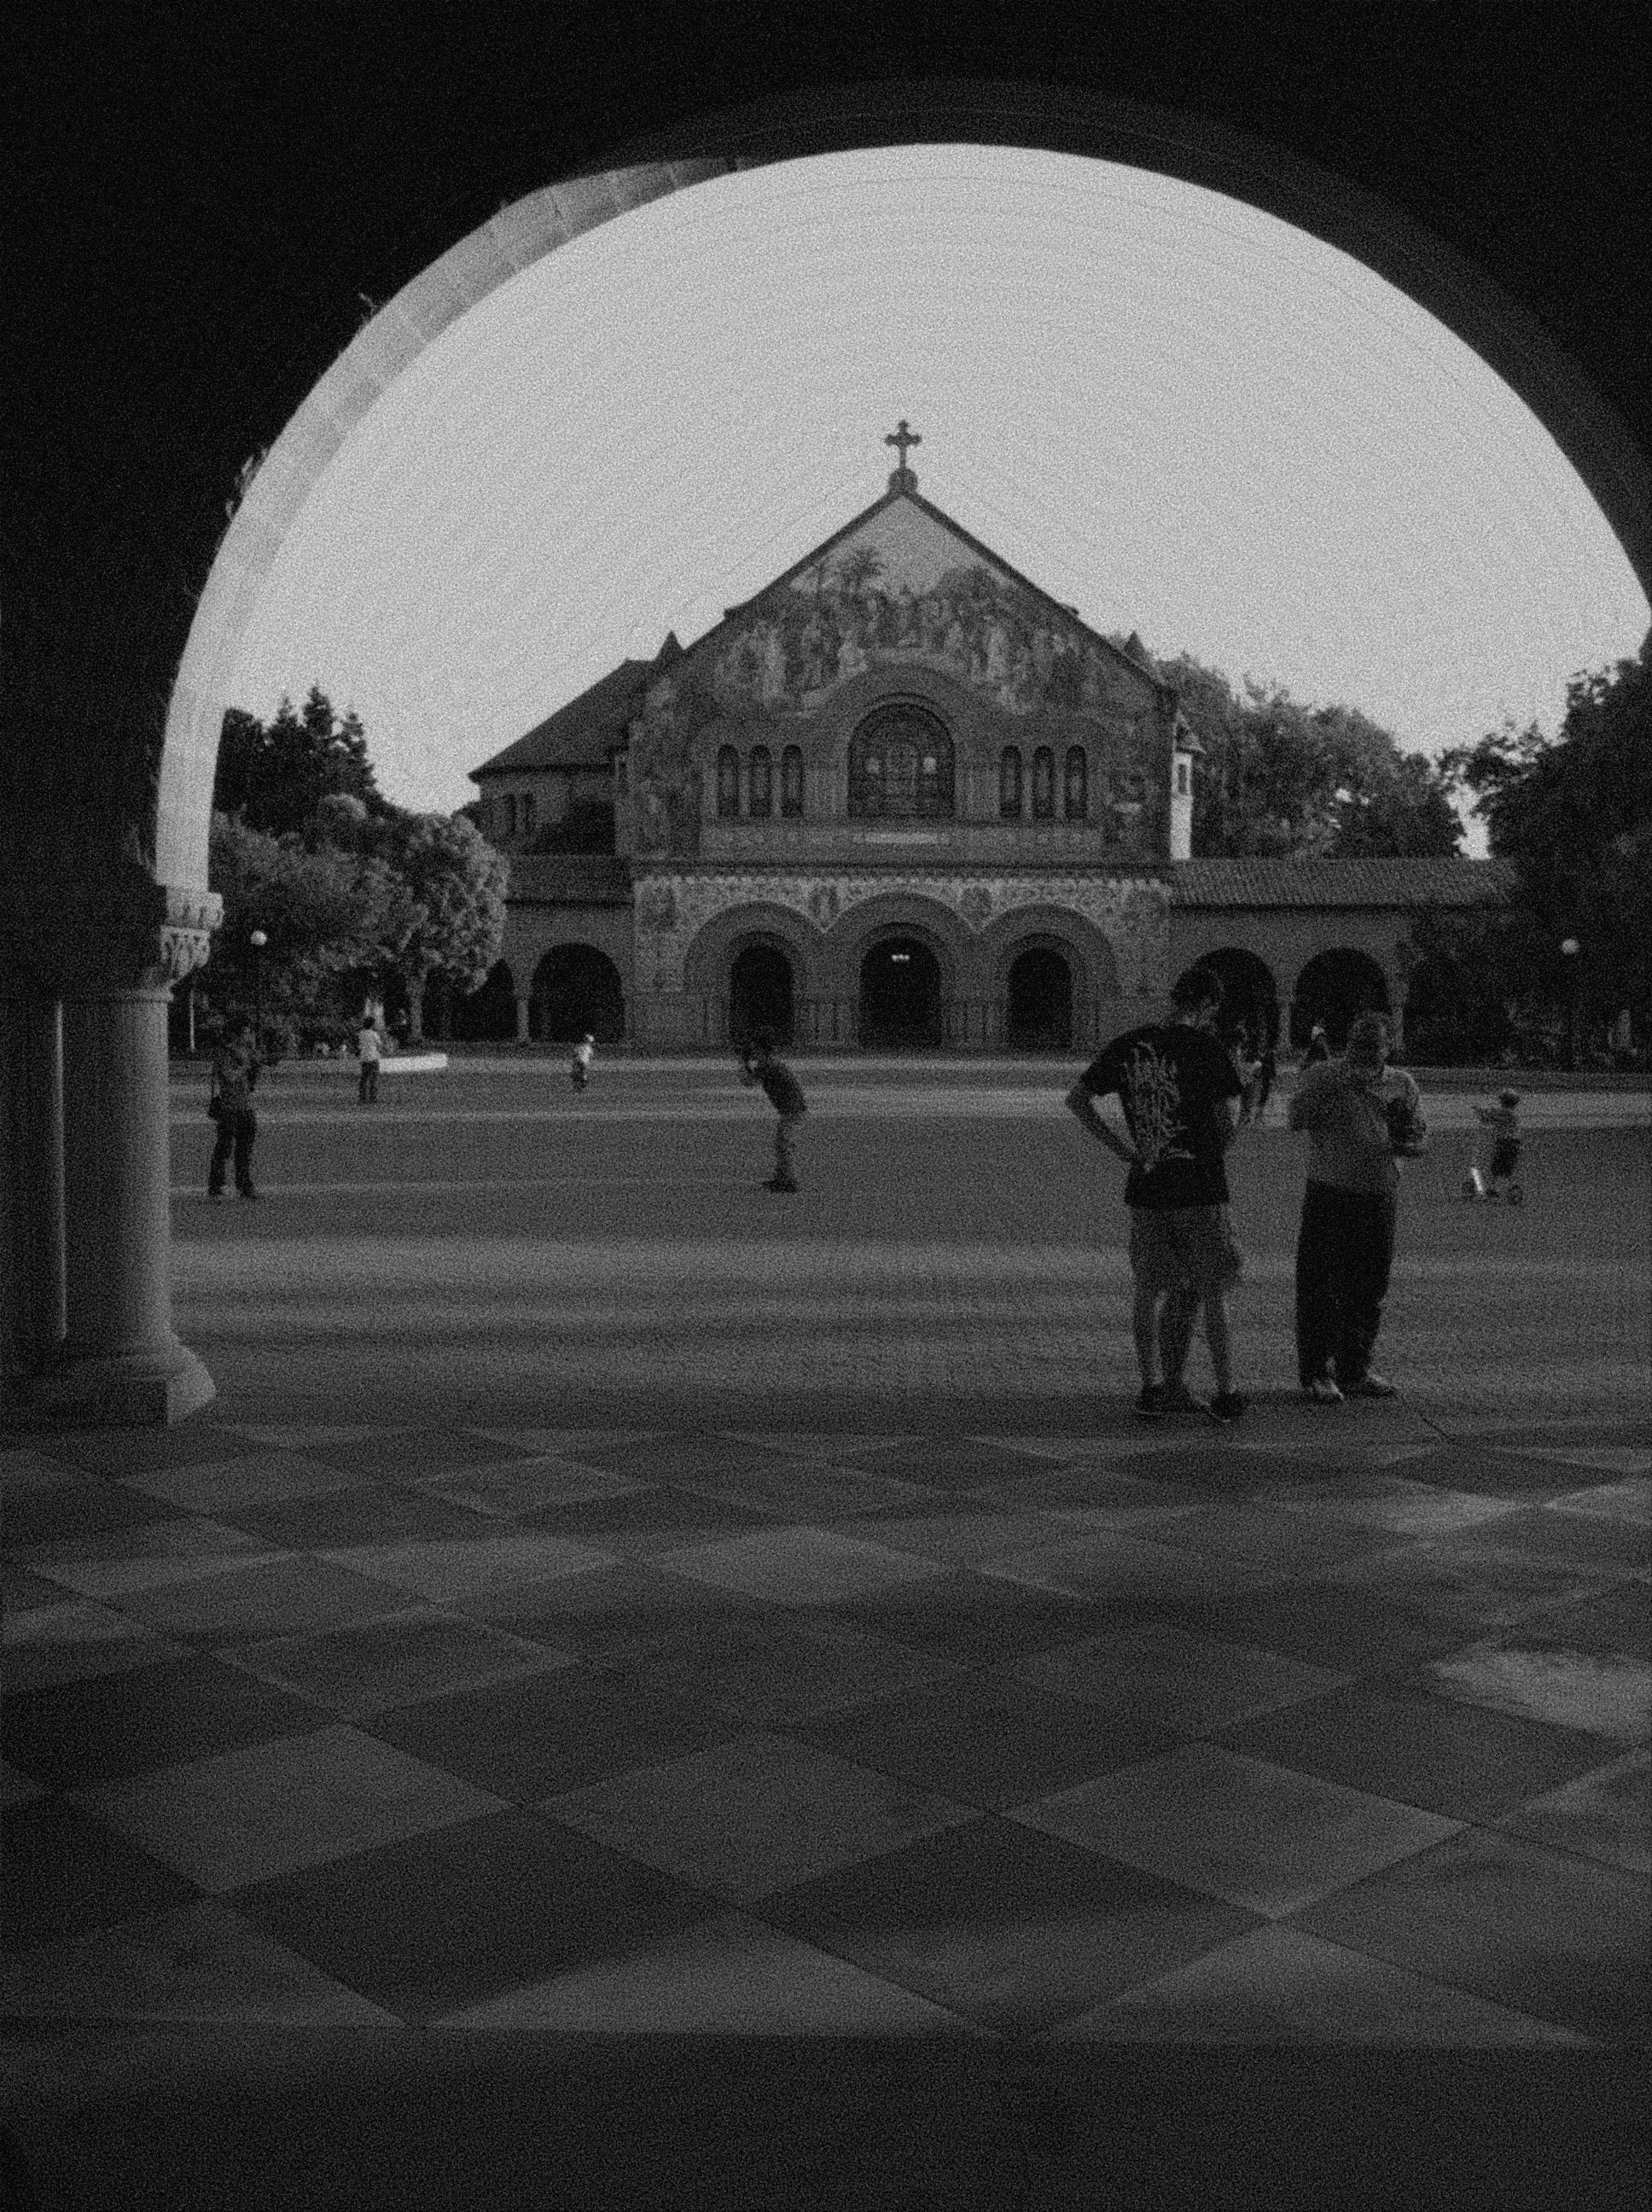
\includegraphics[width=\textwidth]{memchu_wiener_noise.jpg}
                        \caption{Image obtained by using the Wiener filter.\newline $Grad=0.0500$ ; $SSI=0.9979$ ; $JNB=82.926$}
        \end{subfigure}
        \hspace{1cm}
        \begin{subfigure}[b]{0.35\textwidth}
                        \centering
                         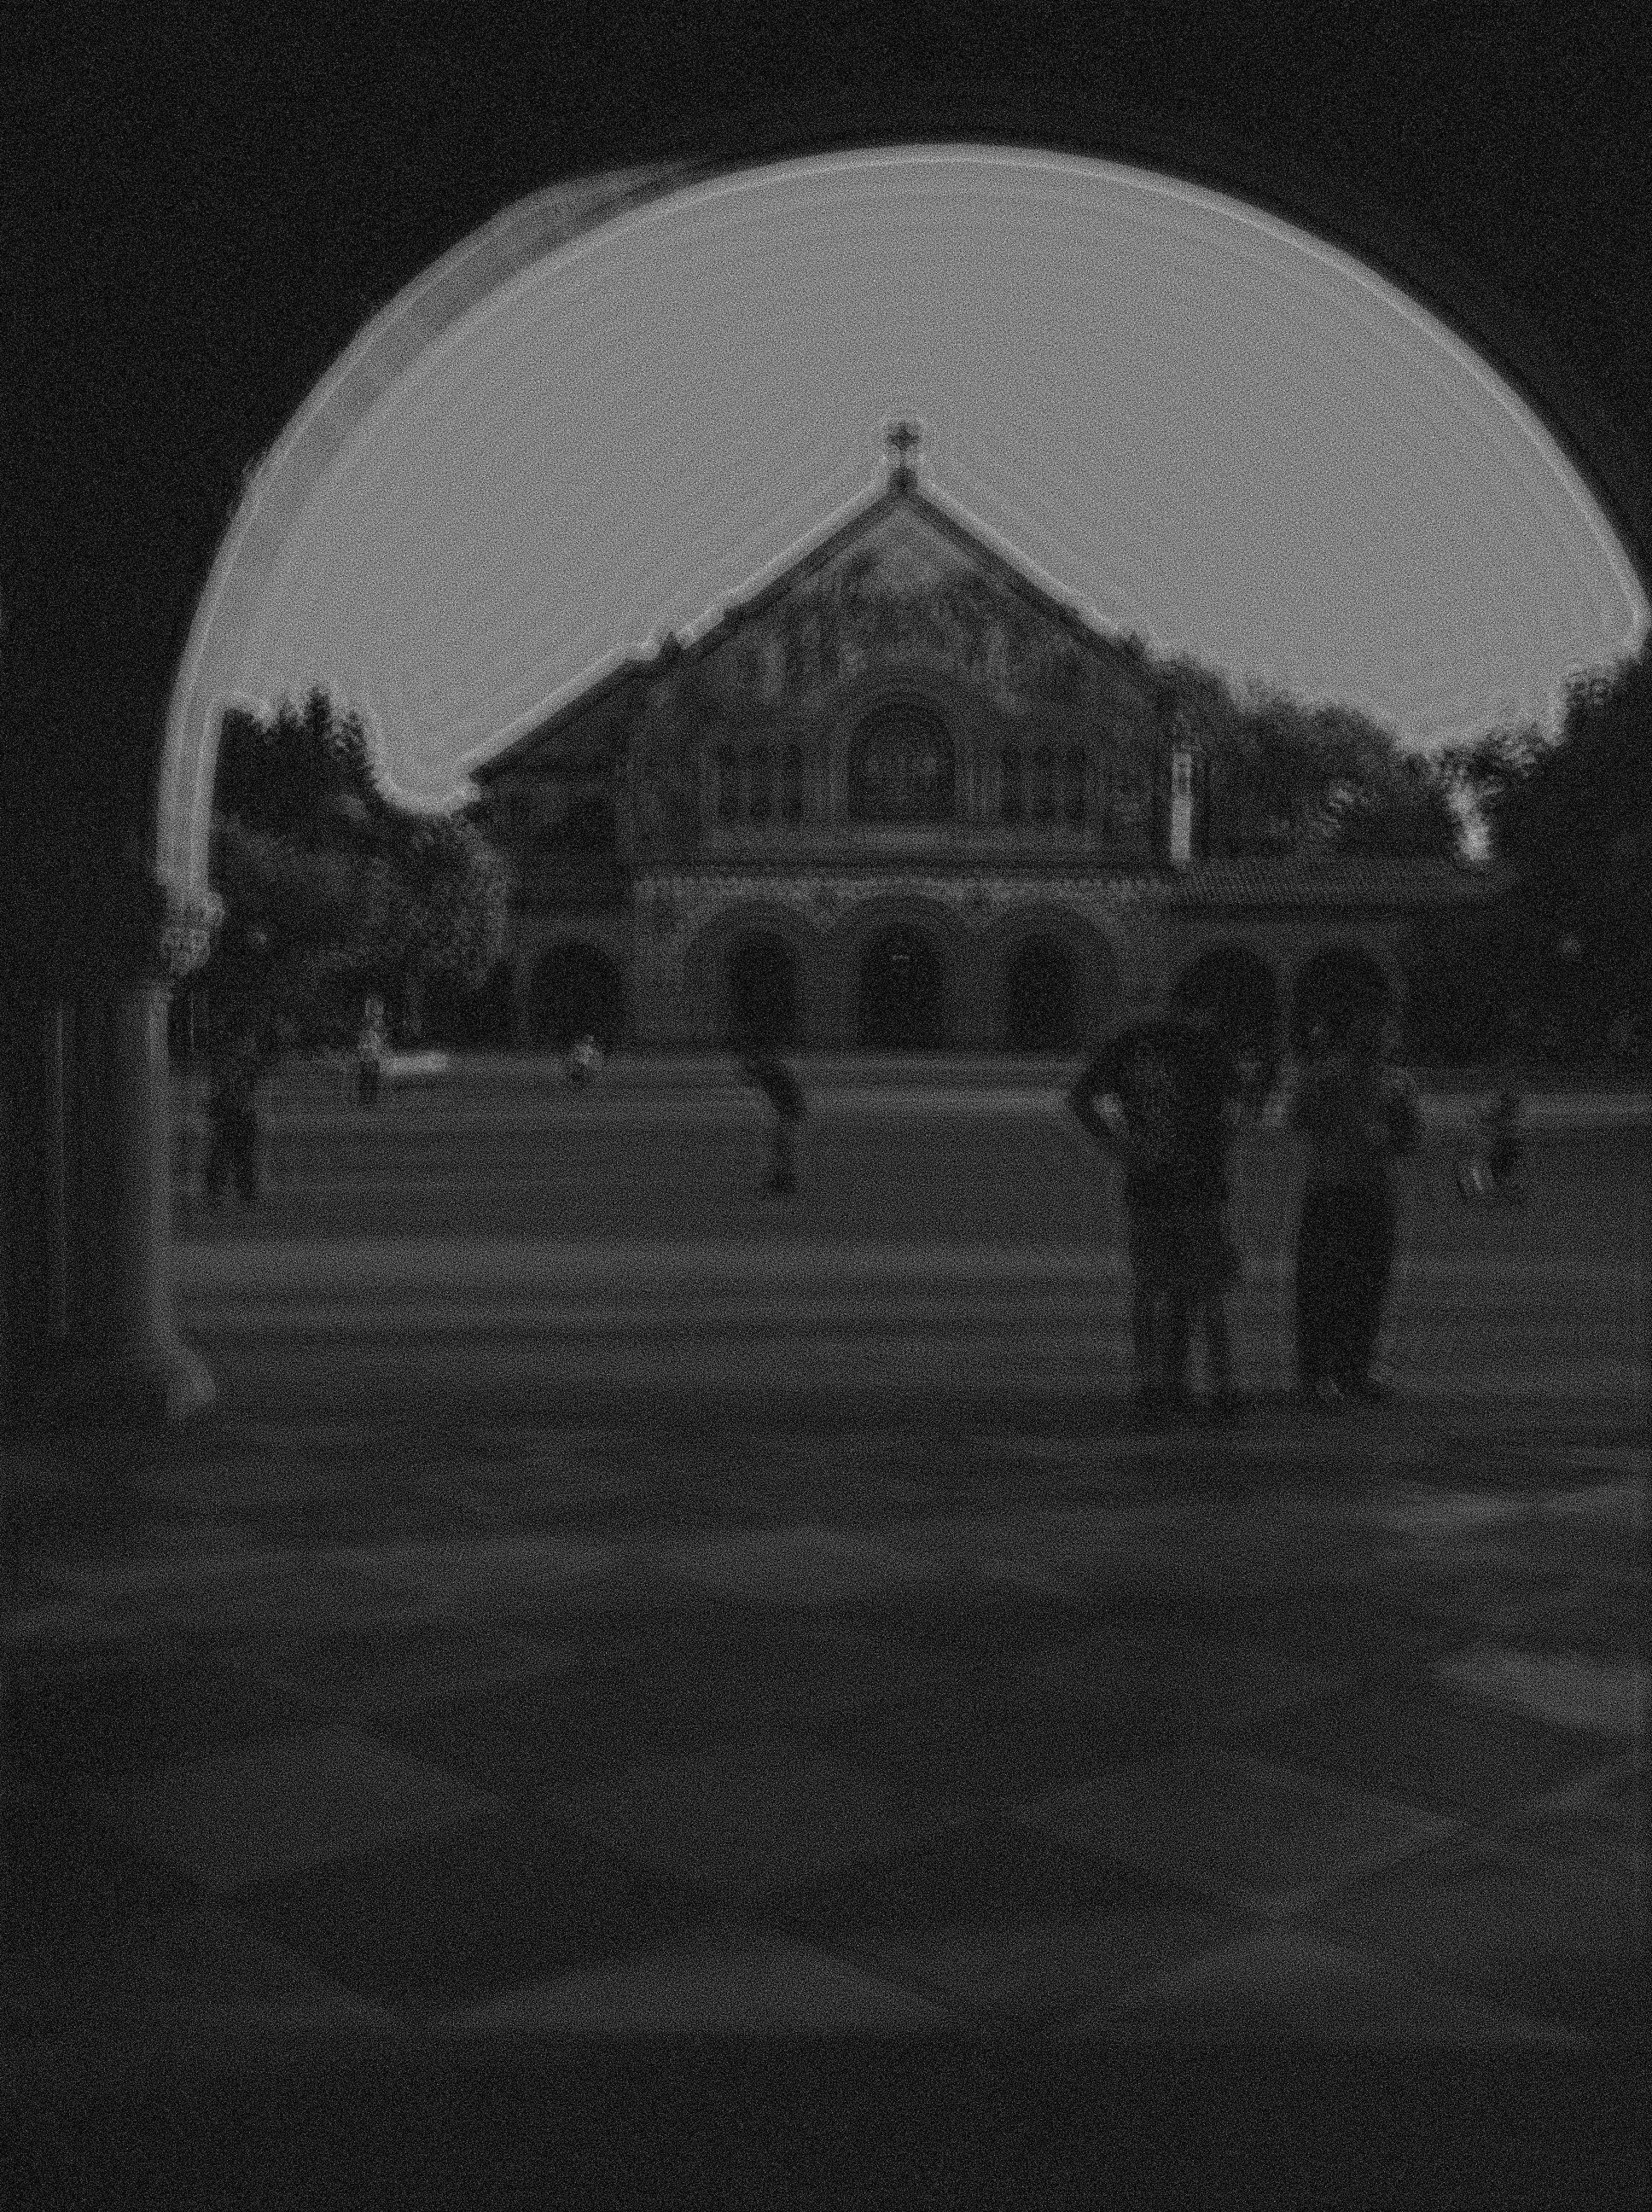
\includegraphics[width=\textwidth]{memchu_geo_noise.jpg}
                         \caption{Image obtained by using the geometric mean filter.\newline $Grad=0.0780$ ; $SSI=0.9924$ ; $JNB=103.011$}
        \end{subfigure} 
        
        \caption{Recovered images using various filters starting with a blurry image with noise (Figure~\ref{fig:base_images_noise}).}
        \label{filtered_images_noise}
\end{figure}

As can be seen from Figure~\ref{filtered_images_nonoise} the filters are able to do a very good job when a good approximation of the PSF is given and there is no noise to interfere with their job. The sharpness metrics were able to perform a good job and the results obtained using them match the visual evidence at the extremes, but are ambiguous otherwise.
The results are very different when noise is introduced into the system, as can be seen from Figure~\ref{fig:base_images_noise}. Even though the PSF and the variance of the noise where known, all the filters had a really hard time sharpening the image, and the one that worked the best is the Wiener filter. This is a common trend that was seen through all the studied cases. In addition, the sharpening metrics are not able to accurately predict sharpness level even at this level of noise, which is minimal compared to real images.

\newpage